\documentclass[11pt, a4paper]{article}

% ===================== PACKAGES =====================
\usepackage[margin=2.5cm]{geometry}
\usepackage[utf8]{inputenc}
\usepackage[T1]{fontenc}
\usepackage{graphicx}
% \usepackage{xcolor}
\usepackage{titlesec}
\usepackage{enumitem}
\usepackage{booktabs}
\usepackage{longtable}
\usepackage{fancyhdr}
\usepackage[hidelinks]{hyperref}
\usepackage{amsmath}
\usepackage{eurosym}
\usepackage{minted} %for code environments
\usepackage{float}
\usepackage{physics} %for real and imag part
\usepackage{amssymb} %for \mathbb
\usepackage[most]{tcolorbox}
\usepackage{wrapfig}
\usepackage[toc,page]{appendix}
%\setlength{\parindent}{0pt}


% ===================== BIBLIOGRAPHY (biblatex + biber) =====================
\usepackage[
    backend=biber,
    style=phys,           % Implementiert den APS/Physical Review Standard
    maxbibnames=3,        % NEU: Wenn es MEHR als 3 Autoren sind, wird gekürzt...
    minbibnames=1,        % NEU: ...und zwar auf den Erstautor (1) plus "et al."
    articletitle=true,    % Titel der Paper anzeigen (gut für längere Arbeiten)
    biblabel=brackets,    % [1] statt 1. im Verzeichnis
    chaptertitle=false,
    pageranges=false,     %
    url=false,            % URLs global ausblenden
    isbn=false,
    doi=true,             % DOIs unbedingt anlassen!
    eprint=true           % arXiv-Links erlauben
]{biblatex}

\AtEveryBibitem{%
  % Prüfen, ob das Feld "eprint" (für arXiv) existiert
  \iffieldundef{eprint}{%
    % FALL 1: KEIN arXiv-Preprint
    \ifentrytype{online}{%
      % Ist eine normale Website -> Nichts löschen, urldate bleibt erhalten!
    }{%
      % Ist ein normales Paper/Buch -> Störfelder löschen
      \clearfield{urldate}%
      \clearfield{url}%
      \clearfield{note}%
      %\clearfield{month}%
    }%
  }{%
    % FALL 2: ES IST EIN arXiv-PREPRINT (eprint ist vorhanden)
    % -> Hier wollen wir das Abrufdatum ebenfalls löschen, 
    % selbst wenn der Typ @online ist.
    \clearfield{urldate}%
    \clearfield{url}% (Meist überflüssig, da der eprint-Link generiert wird)
    \clearfield{note}%
    \clearfield{month}%
    \clearfield{eprintclass}
  }%
}

\addbibresource{references.bib}
% ===================== GLOSSARY (glossaries) =====================
\usepackage[acronym]{glossaries}
\makeglossaries

% ===================== COLORS (adjust to taste) =====================
\definecolor{pulsarblue}{RGB}{20, 60, 110}
\definecolor{pulsargray}{RGB}{75, 75, 75}
\definecolor{codeblue}{RGB}{236, 246, 252}
\definecolor{codeyellow}{RGB}{255, 249, 225}

\newcommand{\code}[1]{\texttt{#1}} %für Programmcode

% ===================== HEADER / FOOTER =====================
\pagestyle{fancy}
\fancyhf{}
\fancyhead[L]{\small MANTIS: MOCS-3D}
\fancyhead[R]{\small \thepage}
\renewcommand{\headrulewidth}{0.4pt}
\title{MANTIS}
\author{Tim Gühring, Leah Haase}
\date{\today}

\begin{document}
% ===========================================================================
%  Titelseite
%
%  Einbinden:  \input{titlepage}   direkt nach \begin{document}
%
%  Benoetigte Pakete in der Praeambel:
%     \usepackage{graphicx}
%     \usepackage{xcolor}
%     \usepackage{hyperref}
%     \usepackage{microtype}   % optional, nur fuer die Sperrung von MANTIS
%
%  Alles Anpassbare steht in diesem Block:
% ---------------------------------------------------------------------------
\definecolor{mantis}{HTML}{1B7A5A}      % Titelfarbe -- hier aendern
\definecolor{subtle}{HTML}{5A5A5A}      % Grauton fuer Nebentext

\newcommand{\ProjectKicker}{Optical Machine Learning Project: MOCS-3D}
\newcommand{\ProjectTitle}{MANTIS}
\newcommand{\ProjectImage}{Chapters/MZI}   % ohne Dateiendung
\newcommand{\AuthorOne}{Tim Gühring}
\newcommand{\AuthorTwo}{Leah Haase}
\newcommand{\RepoURL}{https://github.com/kaschdaniel/MANTIS.git}
% ---------------------------------------------------------------------------

\begin{titlepage}
\centering
\thispagestyle{empty}

\vspace*{\stretch{1.1}}

% ---------- Kicker -------------------------------------------------------
{\normalsize\scshape\color{subtle}\ProjectKicker\par}

\vspace{5mm}

% ---------- Titel zwischen zwei Linien -----------------------------------
{\color{mantis}\rule{0.62\textwidth}{0.9pt}}\par
\vspace{3.5mm}
{\fontsize{54}{54}\selectfont\bfseries\color{mantis}%
 \ifdefined\textls\textls[180]{\ProjectTitle}\else\ProjectTitle\fi\par}
\vspace{7mm}
{\color{mantis}\rule{0.62\textwidth}{0.9pt}}\par

\vspace{16mm}

% ---------- Bild ---------------------------------------------------------
% Faellt auf einen Platzhalter zurueck, solange die Datei fehlt.
\IfFileExists{\ProjectImage.pdf}{%
  \includegraphics[width=0.46\textwidth]{\ProjectImage}%
}{\IfFileExists{\ProjectImage.png}{%
  \includegraphics[width=0.46\textwidth]{\ProjectImage}%
}{%
  \fbox{\parbox[c][0.30\textwidth][c]{0.46\textwidth}{%
    \centering\color{subtle}\itshape\small
    \ProjectImage.png\\[1mm]-- Platzhalter --}}%
}}

\vspace{17mm}

% ---------- Metadaten ----------------------------------------------------
{\Large\scshape Project Report\par}
\vspace{5mm}
{\large\AuthorOne\quad\textcolor{mantis}{\textbullet}\quad\AuthorTwo\par}
\vspace{3mm}
{\large\today\par}
\vspace{3mm}
{\large Friedrich Schiller University Jena\par}

\vspace*{\stretch{1.6}}

% ---------- Fuss: Repository ---------------------------------------------
{\color{subtle}\rule{0.28\textwidth}{0.4pt}\par}
\vspace{3.5mm}
{\small\color{subtle}Source code and data available on\par}
\vspace{1.5mm}
{\normalsize\href{\RepoURL}{%
   \color{mantis}%
   \ifdefined\faGithub\faGithub\hspace{1.2mm}\fi%
   \textbf{GitHub}}\par}

\vspace*{\stretch{0.3}}
\end{titlepage}
\newacronym{ml}{ML}{machine learning}
\newacronym{nn}{NN}{neural network}
\newacronym{pnn}{PNN}{physical neural network}
\newacronym{onn}{ONN}{optical neural network}
\newacronym{mzi}{MZI}{Mach-Zehnder interferometer}
\newacronym{oiu}{OIU}{optical interference unit}
\newacronym{onu}{ONU}{optical nonlinearity unit}
\newacronym{avm}{AVM}{adjoint variable method}
\newacronym{pic}{PIC}{photonic integrated circuit}

%\maketitle
%\textbf{Konvention}
\begin{enumerate}
    \item m: Seitenlänge von downsampled MNIST image
    \item N: Anzahl Channel -> $N=m^2$
    \item theta\_enc: Hyperparameter für scaling von Codierung
    \item thetas, phis: Weights unseres Systems
    \item seed: 1550 Für Reproduzierbarkeit der Datensätze
    
\end{enumerate}

\textbf{Evaluation}
\begin{enumerate}
    \item Position von Detektor-Outputs relevant für Konvergenz?
    \item Input- und Detection-loss einführen (Fiber-loss simulieren)
    \item Detektoren verbinden und obere Hälfte der 1 zuordnen, untere Hälfte der 7? Also mehr Intensität in oberer Hälfte -> 1, andernfalls 7 ?
\end{enumerate}

\textbf{Discussion}
\begin{enumerate}
    \item Stromverbrauch (Unterschied Plug-In Strom und used power)
    \item Begrenzungen: Parameter müssen kontinuierlich sein, außerdem konvergiert gradient-approach nur zum nächsten lokalen Minimum, garantiert nicht globales Minimum \cite{gilesIntroductionAdjointApproach2000}.
    Und Loss-funktion muss für error field diffbar sein
\end{enumerate}

\newpage
\tableofcontents
\newpage
\printglossary[type=\acronymtype]
\newpage

\section{Introduction \& System overview}

%ML is a good alternative to computing the full analytical 
\Gls{ml} has emerged as a powerful paradigm for applications that rely on data-driven optimization, improving system performance by iteratively training on data. Following the introduction of the perceptron by \citeauthor{rosenblattPerceptron1958}, \citeauthor{rumelhartLearningRepresentationsBackpropagating1986} demonstrated that \gls{nn} with hidden layers, trained via backpropagation, can solve non-linearly separable problems such as the XOR problem \cite{rosenblattPerceptron1958,rumelhartLearningRepresentationsBackpropagating1986}. 
This laid the groundwork for a broad range of applications, ultimately enabling the era of transformer-based \cite{vaswaniAttentionAllYou2017} and generative AI models \cite{brownLanguageModelsAre2020a, radfordImprovingLanguageUnderstanding}. 
The performance of such deep-learning models was found to scale predictably as a power law with model size, dataset size, and training compute \cite{kaplanScalingLawsNeural2020, hoffmannTrainingComputeoptimalLarge2022}.
This scaling comes at a substantial energy cost: In 2025 data centers are estimated to account for 1.5\% of global electricity generation, driven increasingly by AI workloads \cite{OurWorldInData, samborskaScalingHowIncreasing2025}.

Photonic hardware offers a promising substrate for running neural networks more efficiently. \citeauthor{cybenkoApproximationSuperpositions1989} and \citeauthor{hornikMultilayerFeedforwardNetworks1989} showed in 1989 that neural networks can approximate any continuous function, given tunable weighted interconnections and non-linear activation functions \cite{cybenkoApproximationSuperpositions1989, hornikMultilayerFeedforwardNetworks1989}. 
Optical systems can provide both. 
As early as 1994, \citeauthor{reckExperimentalRealizationAny1994} demonstrated that any unitary operator can be realized with optical components, enabling arbitrary linear transformations in the optical domain \cite{reckExperimentalRealizationAny1994}. 
Among the various optical neural network (ONN) implementations proposed since, on-chip meshes of \glspl{mzi} stand out for their scalability
\cite{clementsOptimalDesignUniversal2016, shenDeepLearningCoherent2017}. 
Built from single-mode phase shifters and 50:50 beam splitters, such a mesh acts as an \gls{oiu} that carries out the linear part of the computation.
A schematic sketch of the interferometer is shown in Figure \ref{fig:MZI-Phase-shifter}.
The remaining \gls{onu} can be realized through nonlinear optical materials, saturable absorbers, optoelectronic activation, or, as in our system, the intensity detection at the output itself \cite{shenDeepLearningCoherent2017, paiMatrixOptimizationUniversal2019a}.
\begin{figure}[H]
    \centering
    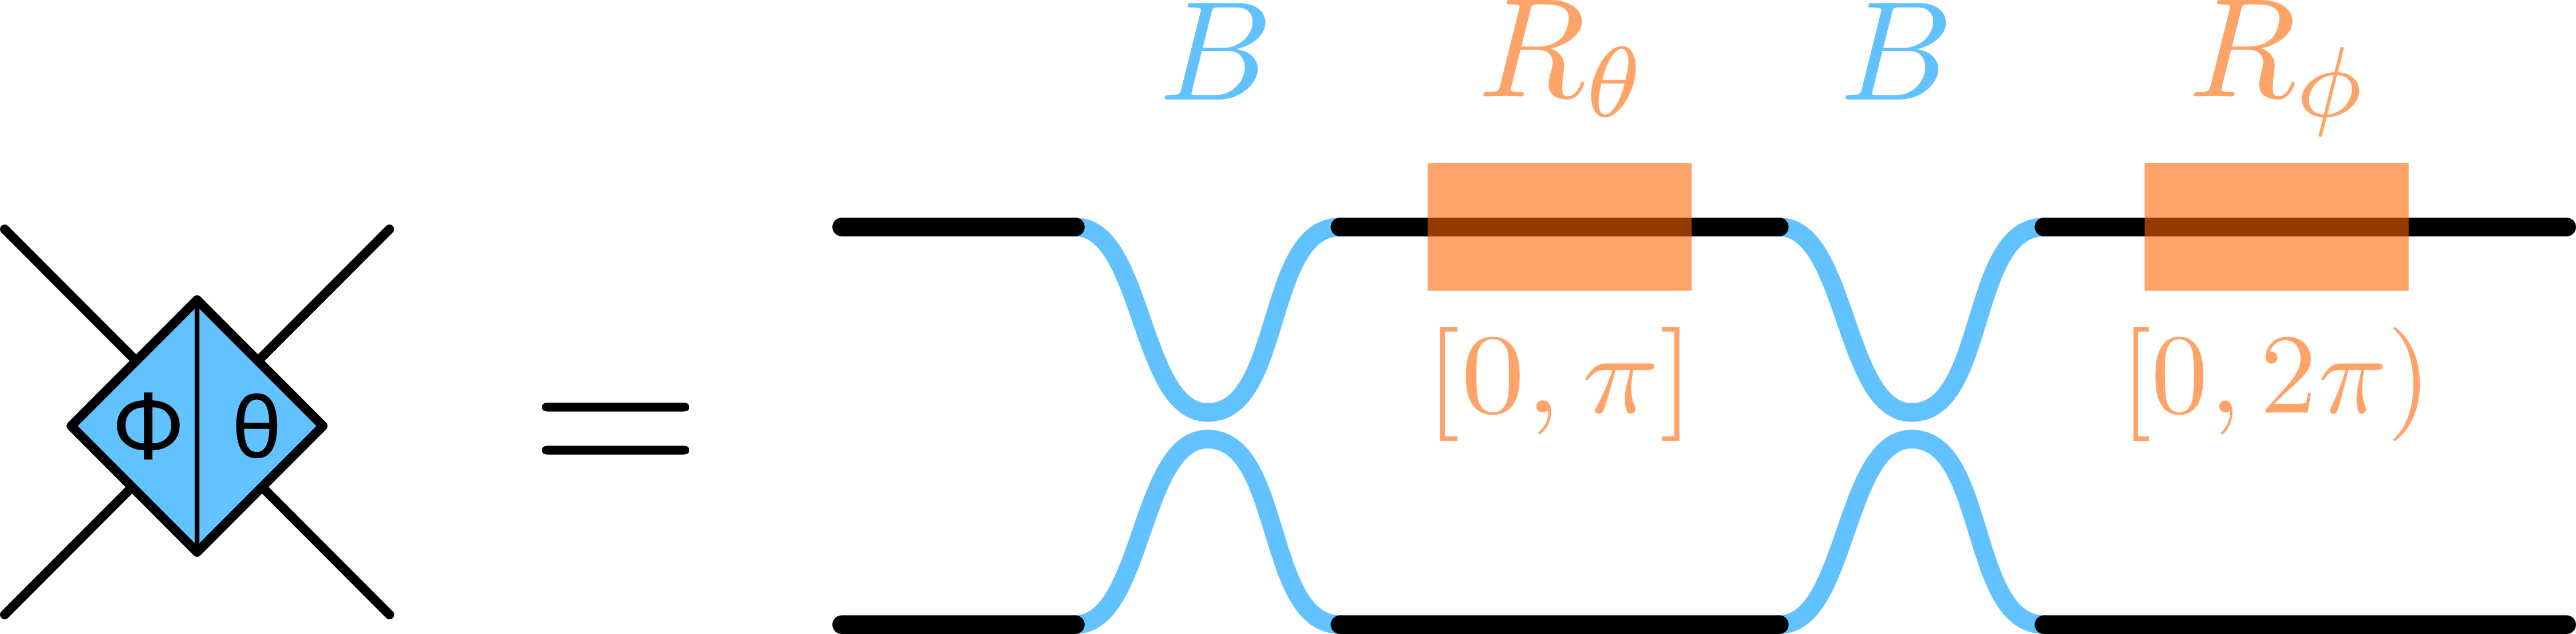
\includegraphics[width=0.5\linewidth]{images/MZISchematics.png}
    \caption{Illustration of a \gls{mzi} composed of beam splitters $B$ and phase shifters $R$. The \gls{mzi} is uniquely characterized by its internal and external phase shift parameters $\theta$ and $\phi$. The black lines represent single mode waveguides, forming the beam splitter using directional coupling.}%nach Miller
    \label{fig:MZI-Phase-shifter}
\end{figure}

%What is training
Training a \gls{nn} means adjusting its parameters such that its predictions match the true result as closely as possible.
This is formalized through a loss function $\mathcal{L}$, which quantifies the discrepancy between the network output and the desired output for a given input.
Training then reduces to a minimization problem: the parameters are iteratively updated along the negative gradient of $\mathcal{L}$ until a minimum is reached.
The practical feasibility of this scheme rests on the backpropagation algorithm \cite{rumelhartLearningRepresentationsBackpropagating1986}.
By applying the chain rule from the output layer backwards, the derivatives with respect to all parameters are obtained in a single pass.
This prevents the cost of a full gradient evaluation from growing with the number of parameters.

%What is Gradient-descent training through physical dynamics
The matrix--vector products required for training can be executed on the physical system itself \cite{hermansTrainableHardwareDynamical2015}. 
Propagating an error field backwards through the device then yields the gradient needed for gradient descent. 
This error field is determined by the deviation of the output from the desired result. 
The central advantage of adjoint-based backpropagation, used in this work, is its scaling~\cite{hughesAdjointMethodInverse2018}. 
The cost of a full gradient evaluation is independent of the number of parameters. 
On hardware, three in-situ intensity measurements after each phase shifter suffice to recover the gradient for all parameters at once. 
Every parameter can then be updated simultaneously to approach a local minimum of the loss landscape. 

The objective of this work is to implement a binary classifier using the \gls{mzi} mesh as the physical core. The model will be trained with samples of handwritten digits ``1'' and ``7'' from the MNIST dataset, using the adjoint-based backpropagation. After the processing layer, two detectors at arbitrary channels will measure the intensity and make a prediction based on the winner-takes-it-all principle. The complete setup is shown in Figure \ref{fig:Objective-Scheme}.
We expect to achieve a high testing accuracy with both the linear regression and the optical model.
In contrast to the linear regression, the optical model has a non-linearity at the detection, which might be an advantage for non-linearly separable problems.
%Expectation?
%The ...
%Und dann kommt noch ein Statement zu den objectives und den expected outcomes
%Objectives: Binäre unterscheidung von handgeschriebenen Ziffern (mnist-dataset)
%(\ref{fig:Objective-Scheme}, MNIST Dataset wird in Vektor zerhackt, geht in input layer, geht durch die Transfer-Matrix, geht in die Detektoren)\\
%Benchmark gegen lineare regression
\begin{figure}[H]
    \centering
    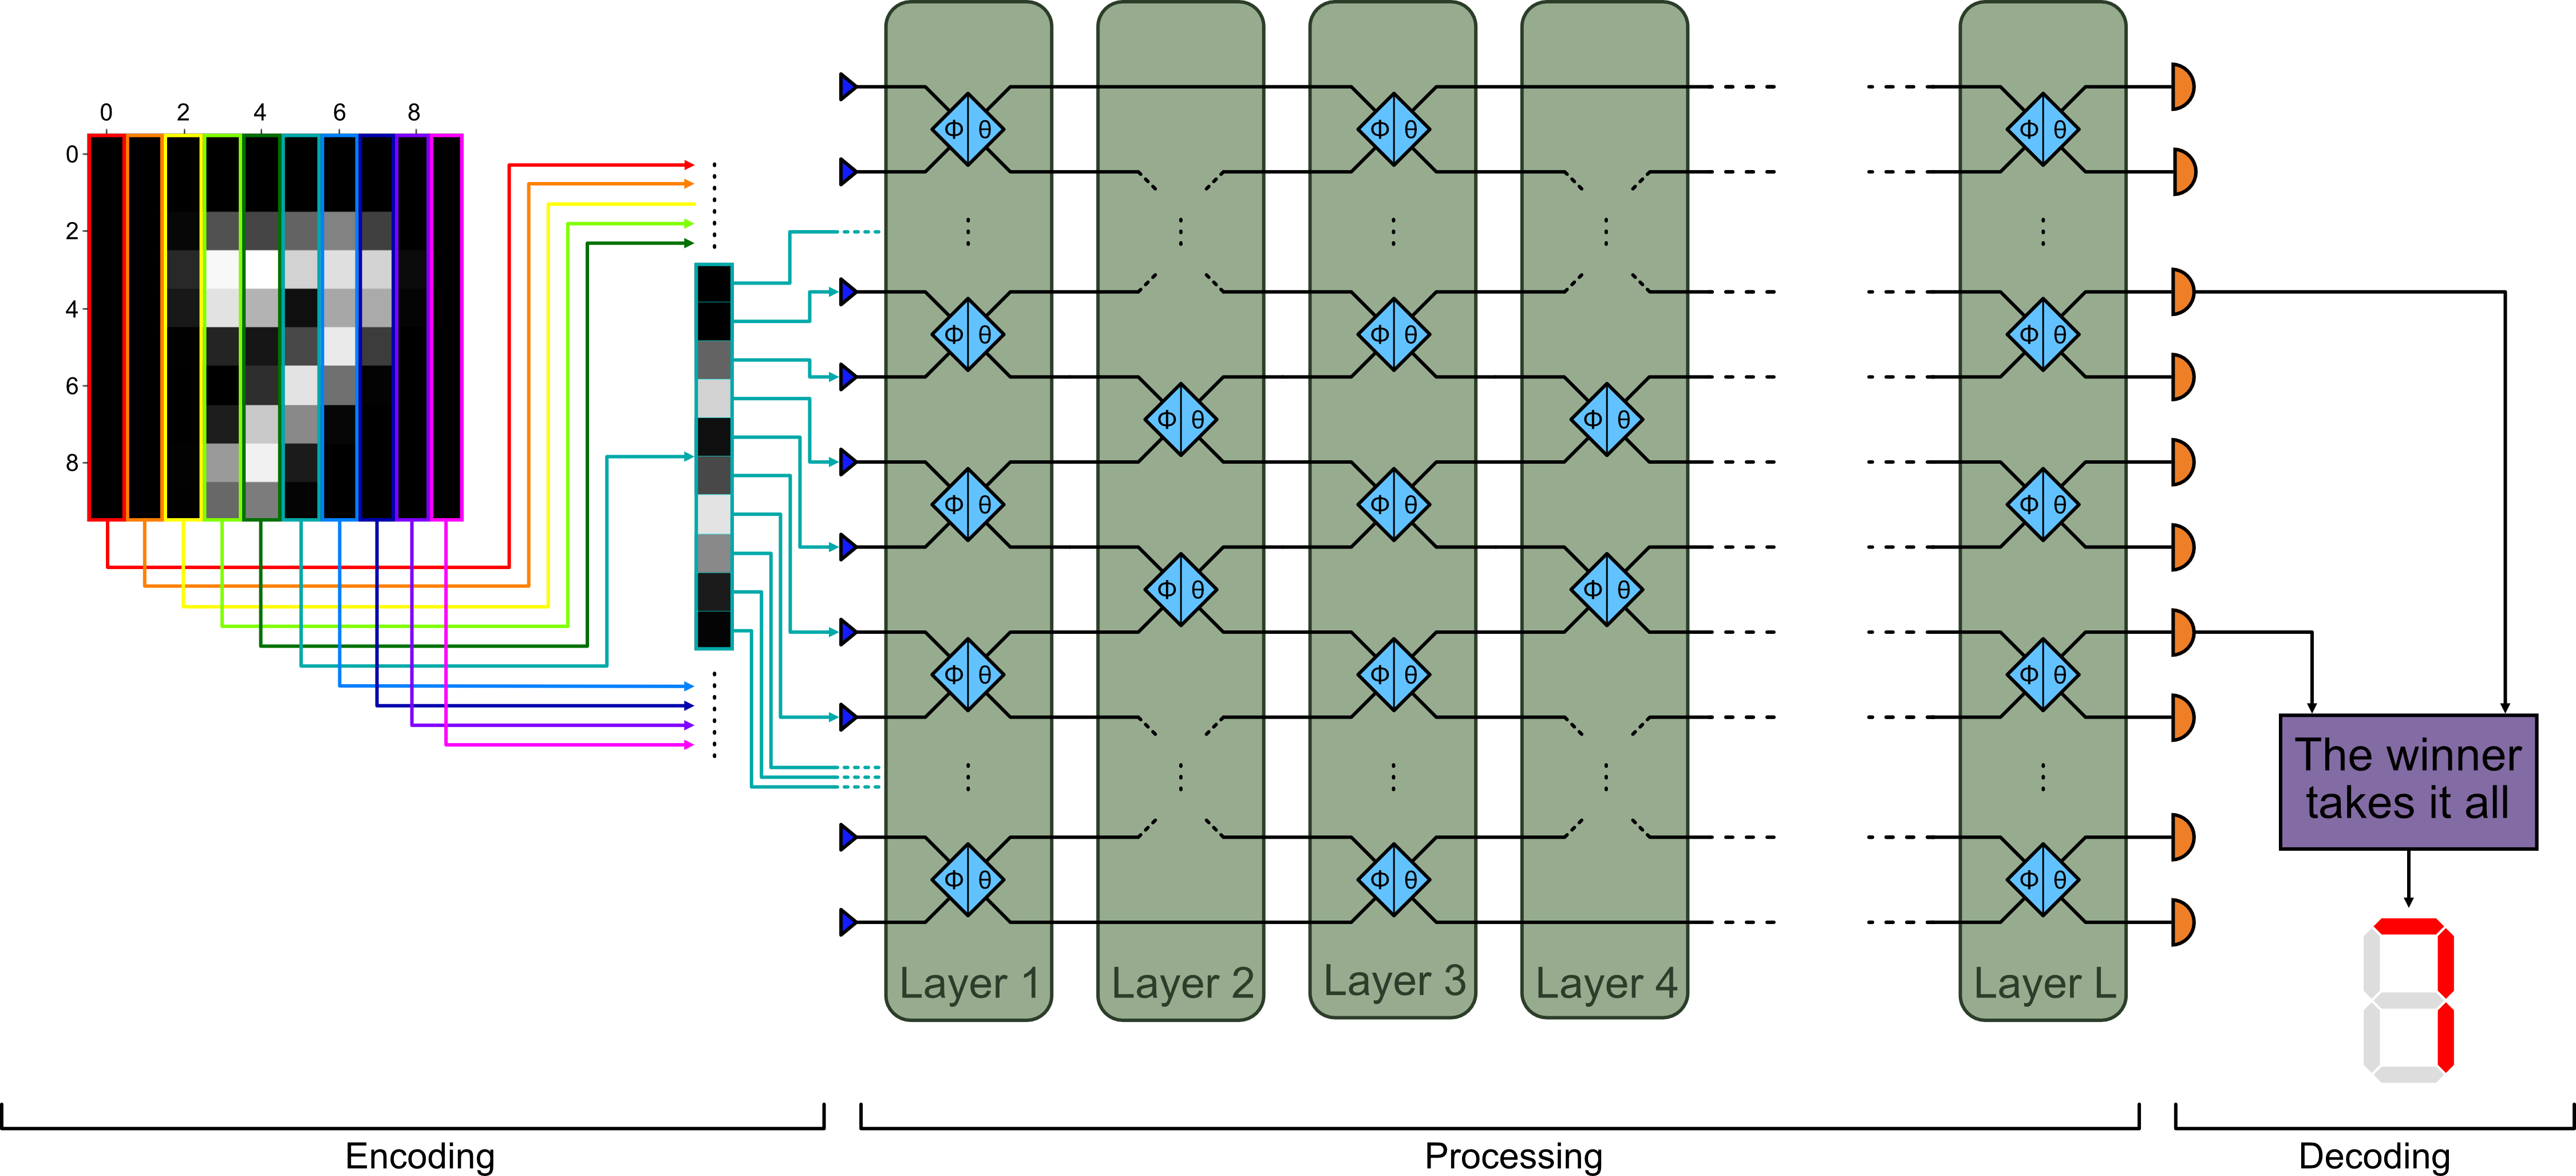
\includegraphics[width=1\linewidth]{images/EncodingProcessingDetectionScheme.png}
    \caption{Scheme illustrating the encoding, processing and decoding steps in the optical model for an image of the MNIST dataset.}
    \label{fig:Objective-Scheme}
\end{figure}
%Expected Outcomes: Mention linear regression, erwarten benefit durch non-linearity am ende (?)
%Außerdem 
%Mention energy-consumption scaling depending on neuron number?
%--> Way more energy-efficient and speed-up

%Vielleicht genauere Einordnung, für welche ML Anwendungen dieser Ansatz gut geeignet ist,... wieso 


%Aus der gegebenen PDF:
%Brief descrip3on of chosen op3cal system and training approach
%Clear statement of objec3ves and expected outcomes
%1 page

\section{System implementation} 
%3-5 pages
\subsection{Loading and preprocessing MNIST data}
The MNIST dataset is loaded in the function \code{get\_data} in file \code{encoding.py} using the function \code{keras.datasets.mnist.load\_data}. The images depicting the digits ``1'' and ``7'' are selected. Using the \code{get\_data} function, the desired number of samples can be specified and the distribution of both digits in the dataset can be balanced. The split ratio of the dataset in training and testing data can be chosen as well, with a default value of 0.8.
The images have a side length of 28\,px and are down-sampled using the \code{skimage.transform.resize} function in the function \code{down\_sample}. The default side length is 10\,px.
Then, the images are reshaped to an one-dimensional vector and normalized using the function \code{reshape\_and\_normalize}. The principle of the reshaping is illustrated in Figure \ref{fig:Objective-Scheme}.
%- with the argument \code{number} of the function \code{get\_data}, you can set the desired size of the sample-set.
%- Since the MNIST pool is slightly imbalanced (6742 ones vs 6265 sevens in the training split), taking all samples or choosing randomly would put the majority-class baseline towards 52.5\%. To prevent this inequality, the argument \code{balanced} enforces an equal count of every digit.
Furthermore, the energy in each image vector can be normalized in the function \code{get\_data} by dividing it by its norm.

\subsection{Linear Regression}
The linear regression is implemented using the Moore-Penrose pseudoinverse in the function \code{linear\_regression} in \code{baseline.py} (see Fig. \ref{code:lin-reg}).
Based on predicted labels \code{y\_pred} and the true labels, the confusion matrix and the accuracy for the binary classification are calculated.

\begin{figure}[H]
\centering
\begin{minted}
[
frame=none,
framesep=2mm,
baselinestretch=1.2,
bgcolor=codeyellow,
fontsize=\footnotesize,
linenos
]{python}
F = np.vstack([np.ones(len(X_train.T)), X_train]).T
theta = np.linalg.pinv(F) @ y_train

y_pred = theta[0] + np.sum(theta[1:] * X_test.T, axis = 1)
y_pred_label = (y_pred >= 0.5).astype(np.float64)
\end{minted}
\caption{Excerpt from function \code{linear\_regression} in \code{baseline.py}.}\label{code:lin-reg}
\end{figure}

\subsection{Optical Machine Learning}
\subsubsection{Encoding}
To encode information optically, we use the electromagnetic wave propagating through the wave-guide channels of the \gls{mzi} mesh. 
Since Maxwell's equations couple the electric and magnetic fields, it is sufficient to describe the wave by one of them, and therefore we work with the electric field throughout. 
For a monochromatic wave of angular frequency $\omega$ propagating along the waveguide axis with wave vector $\vec{k}$, the field in mode $j$ can be written as:
\begin{align*}
    E_j(\vec r, t) = A_j(\vec r)\, e^{i(\vec k \cdot \vec r + \omega t)}.
\end{align*}
Here we consider only a single scalar component of the field with amplitude $A_j$, omitting the vector character.
This is justified since we assume that all channels carry the same guided mode with a fixed polarisation.
For an uniform chip architecture, the channels acquire the exact same phase by propagating along the optical axis. Since the information is carried by the relative differences between the channels, we express the relevant components by 
\begin{align*}
    \mathbf{E}(\vec{r}, t) = e^{i(\vec{k} \cdot \vec{r} +\omega t)}
    \begin{pmatrix}
        A_1(\vec r)\, e^{i\varphi_1} \\ \vdots \\ A_m(\vec r)\, e^{i\varphi_m}
    \end{pmatrix},
\end{align*}
where $\varphi_j$ represents the initial phase given to the electric field in mode $j$.
The state of the system is therefore fully described by this vector of complex amplitudes, which is the quantity propagated in our simulation.
\\
The pixel values $V(x,y)$ of an image are imprinted on this field by modulating either the amplitudes $A_j$ or the initial phases $\varphi_j$ (see Fig. \ref{code:encoding}).
When applying amplitude encoding, the normalized pixel values are mapped onto the field
amplitudes while the phase is kept constant, with $E_j = \theta \, V_j$ and $\varphi_j = 0$.
%\begin{align*}
%    E_j = \theta \, V_j , \qquad \varphi_j = 0.
%\end{align*}
Phase encoding is an alternative in which the pixel values are mapped onto $\varphi_j$ at constant amplitude.
The hyperparameter $\theta$ is controlling the encoding strength.
%, is discussed as an alternative in Section~\ref{sec:AmplitudeEncoding}.

\begin{figure}[H]
\centering
\begin{minted}
[
frame=none,
framesep=2mm,
baselinestretch=1.2,
bgcolor=codeyellow,
fontsize=\footnotesize,
linenos
]{python}
def amplitude_encoding(image, theta_enc=1):
    """Encode image information in amplitude of electric field."""
    return (image * theta_enc).astype(complex)

def phase_encoding(image, theta_enc=1):
    """Encode pixel values in the phase, constant amplitude."""
    return np.exp(1j * theta_enc * np.pi * image)
\end{minted}
\caption{Excerpt from \code{encoding.py} showing the functions \code{amplitude\_encoding} and \code{phase\_encoding}.}\label{code:encoding}
\end{figure}

\subsubsection{Processing}
The processing is done by the \glspl{mzi} in the mesh, that can be set to perform any unitary transformation on the electric fields in each channel \cite{reckExperimentalRealizationAny1994}.
Consisting of an arrangement of beam splitters $B$ and phase shifters $R$ (see Figure \ref{fig:MZI-Phase-shifter}), the \gls{mzi} implements any arbitrary Givens rotation $T=R_\phi B R_\theta B$:
\begin{align*}
    T=\frac{1}{2} \begin{pmatrix}
    e^{i\phi} & 0 \\
    0 & 1
    \end{pmatrix}\begin{pmatrix}
    1 & i \\
    i & 1
    \end{pmatrix}\begin{pmatrix}
    e^{i\theta} & 0 \\
    0 & 1
    \end{pmatrix}
    \begin{pmatrix}
    1 & i \\
    i & 1
    \end{pmatrix}.
\end{align*}
Permutating their placements in the mesh along the layers allowing mixing between all channels, builds the \gls{oiu} that can form any unitary operation.
Applying these rotations block-wise to their respective channels, this yields the transfer-matrix of layer $L$, allowing the full propagation by matrix multiplication.
\begin{align}
    \mathbf{E_{out}}=\hat{W}_L\hat{W}_{L-1}...\hat{W}_1\mathbf{E_{in}}=\hat{W}\mathbf{E_{in}}.
    \label{eq:layerwisepropagation}
\end{align}
Note that a layer here refers to the depth of one \gls{mzi} (2 beam splitters and 2 phase shifters) and is not to be confused with the definition of one layer for the adjoint-based backpropagation. There each layers is representing one tunable parameter (1 beam splitter and 1 phase shifter).

Accordingly, the transfer matrices are calculated using functions \code{beamsplitter}, \code{phase\_shift} and \code{U} (see Fig. \ref{code:transfer-matrices}).
Additionally, two functions \code{U\_theta} and \code{U\_phi} are defined which allow a separate calculation of the transfer matrices for each combination of a phase shifter and beam splitter separately for the gradient-descent algorithm.

\begin{figure}[H]
\centering
\begin{minted}
[
frame=none,
framesep=2mm,
baselinestretch=1.2,
bgcolor=codeyellow,
fontsize=\footnotesize,
linenos
]{python}
def beamsplitter(eta=1.0):
    """Transfer matrix of a beamsplitter with power transmission eta."""
    B_ideal = (1/np.sqrt(2)) * np.array([[1, 1j],
                                         [1j, 1]], dtype=np.complex128)
    return np.sqrt(eta) * B_ideal

def phase_shift(alpha): 
    """Transfer matrix to apply a phase shift to upper mode."""
    return np.array([[np.exp(1j*alpha), 0],
                     [0, 1]], dtype=np.complex128)

def U(theta, phi, eta=1.0):
    """Transfer matrix of the MZI with phase shifts theta and phi. 
    eta: Power transmission per beamsplitter. Two beamsplitters per MZI."""
    B = beamsplitter(eta)
    return phase_shift(phi) @ B @ phase_shift(theta) @ B
\end{minted}
\caption{Excerpt from \code{mesh.py} showing the functions \code{beamsplitter}, \code{phase\_shift} and \code{U}.}\label{code:transfer-matrices}
\end{figure}

The class \code{MZIMesh} is a central part of the processing (see Fig. \ref{fig:class-MZIMesh}). It allows the definition of the chip structure. 
The implemented options include a rectangular and a triangular mesh of \gls{mzi}s.
According to \citeauthor{paiMatrixOptimizationUniversal2019a}, convergence can be vastly accelerated by using the correct initialization. The ``Haar initialization'' introduced in \cite{paiMatrixOptimizationUniversal2019a}, is based on globally approximating a uniformly random unitary matrix rather than just randomizing individual components. Thus, position-dependent \gls{mzi} split ratios form a global Haar-random matrix, ensuring that input light is evenly distributed across all spatial modes.
The code for the generation of the rectangular mesh is shown in Figure \ref{code:rect-mesh} as an example.
Parameters, like the values of \code{theta} and \code{phi} for each phase shifter are stored separately. 

\begin{figure}[H]
    \centering
    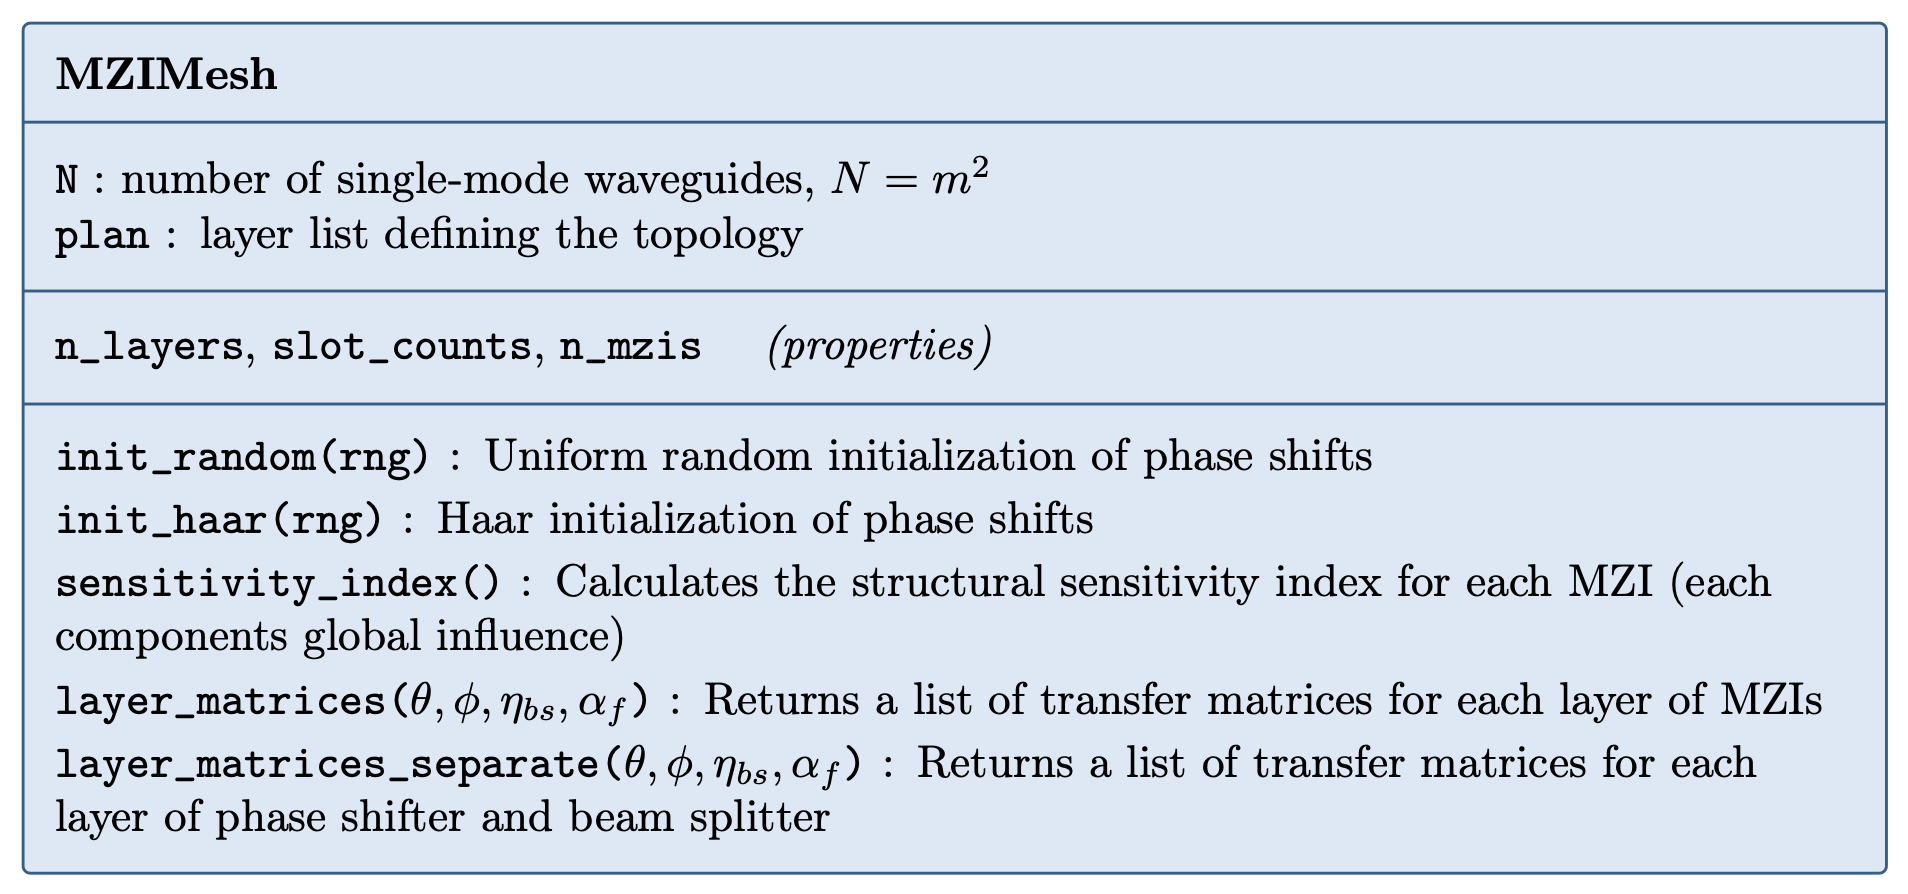
\includegraphics[width=0.7\linewidth]{images/main_classdiagram_mesh.png}
    \caption{Class diagram for class MZIMesh from mesh.py}
    \label{fig:class-MZIMesh}
\end{figure}

\begin{figure}[H]
\centering
\begin{minted}
[
frame=none,
framesep=2mm,
baselinestretch=1.2,
bgcolor=codeyellow,
fontsize=\footnotesize,
linenos
]{python}
def plan_rectangular(N, L):
    """Clements / rectangular mesh: L Layers, with alternating offset 0 and 1.
    Universal for L = N. Returns: list of ("mzi", ks)."""
    plan = []
    for l in range(L):
        start = l % 2
        ks = list(range(start, N - 1, 2))
        plan.append(("mzi", ks))
    return plan
\end{minted}
\caption{Excerpt from \code{mesh.py} showing the function \code{plan\_rectangular}.}\label{code:rect-mesh}
\end{figure}

The functions which are most relevant for the propagation of the electric field in the chip are summarized in Figure \ref{code:propagation}.
The function \code{forward} returns the electric field at the output ports of the chip on the right, when an electric field has entered through the input ports on the left, while the function \code{backward} gives the output field for the reverse propagation direction from the right to the left.
The output of the forward propagation is calculated by applying the transfer matrix $\hat{W}_L$ of each layer which are stored in \code{layers} to the incoming electric field vector.
For the backward propagation the transfer matrices are transposed and their order is reversed, then they are applied to the electric field vector incoming from the right.

\begin{figure}[H]
\centering
\begin{minted}
[
frame=none,
framesep=2mm,
baselinestretch=1.2,
bgcolor=codeyellow,
fontsize=\footnotesize,
linenos
]{python}
def forward(E_in, layers):
    """Forward propagation through given layers."""
    for Ml in layers:
        E = Ml @ E
    return E

def backward(lam_out, layers):
    """Backward propagation through reversed layers."""
    return forward(lam_out, adjoint_layers(layers))

def adjoint_layers(layers):
    """Transposing layers and reversal of their order."""
    return [Ml.T for Ml in reversed(layers)]
\end{minted}
\caption{Shortened excerpt from \code{processing.py} showing the functions \code{forward}, \code{backward} and \code{adjoint\_layers} which are relevant for the electric field propagation through the chip.}\label{code:propagation}
\end{figure}

\subsubsection{Decoding}
The detected intensity is calculated as the absolute squared value of the electrical field for each output:
$I_n=|E_{out,n}|^2=E_{out,n}\cdot E_{out,n}^*$.
Two specific output ports are assigned to digits ``1'' and ``7'' respectively.
The digit assigned to the port with the higher intensity is returned as the predicted label. This is implemented in the functions \code{detection} and \code{\_detector\_scores} in \code{decoding.py}.

\subsubsection{Gradient-Descent Training Through Adjoint-based Backpropagation}
Conventional backpropagation operates on a known computational graph and requires the transpose of each weight matrix to be available as an explicit numerical object. 
In our system the weights are not numbers stored in memory but the phase settings of the \glspl{mzi}, and the linear operation they implement is a propagating optical field.
What is therefore needed is a formulation of the same gradient in terms of the physical parameters of the device.

The \gls{avm} provides exactly this formulation. 
It originates in the calculus of variations and was later adapted to engineering sensitivity analysis. 
Today it is a standard tool of photonic inverse design
\cite{gilesIntroductionAdjointApproach2000, veronisMethodSensitivityAnalysis2004, moleskyInverseDesignNanophotonics2018}.
Its key result is that the derivative of a scalar figure of merit with respect to all design parameters follows from only two field solutions. 
The first is the original field, driven by the physical input source. 
The second is an adjoint field, driven by a source that encodes the error at the output \cite{hughesAdjointMethodInverse2018}. 
The gradient with respect to an individual parameter is then given by the local overlap of these two fields at its position.
For the calculation of the gradient, we use the following equation, which is derived in appendix \ref{appendix:derivation}:
\begin{align}
    \frac{\mathrm{d}\mathcal{L}}{\mathrm{d}p}
    = -2\,\Im\left\{ A_p\,A_p^{\mathrm{adj}} \right\}
    \label{eq:final1}
\end{align}
%\paragraph{Algorithmic Implementation in \code{trainer} class}\mbox{}\\
Summarizing this derivation, that is specifically matched to our system, we get the following practical procedure for our training:
%(In our software based simulation, we...)
\begin{enumerate}
    \item Propagating the input field $\mathbf{E}_{in}$ (encoded MNIST data) using forward propagation according to equation \eqref{eq:layerwisepropagation}. After every phase shifter ($\phi$ and $\theta$), the electrical field in that channel is stored in a list.
    \item Decoding the output and calculating the loss for the chosen cost function. Determining the adjoint vector for the backpropagation.
    \item Propagating the adjoint field using backward propagation through the transposed layer transfer matrices. After every phase shifter ($\phi$ and $\theta$), the electrical field in that channel is stored in a list.
    \item Calculating the derivative of the loss with respect to each phase shifter using equation \eqref{eq:final1} by interfering the forward and backward propagated fields at each position.
    The parameters $\phi$ and $\theta$ are updated accordingly using gradient-descent.
\end{enumerate}

%\subsection{Zusammenfassung des Trainingsschritts}

%Ein vollständiger Gradientenschritt besteht damit aus vier Operationen:

%\begin{enumerate}
%  \item Propagation des kodierten Eingangsfeldes $\mathbf{E}_0$ durch das Mesh
%        gemäß \eqref{eq:layerwisepropagation} unter Speicherung der Feldamplituden nach jeder
%        Layer-Ebene.
%  \item Auswertung der Detektorintensitäten \eqref{eq:detection}, der
%        Kostenfunktion $\mathcal{L}$ und der adjungierten Quelle
%        \eqref{eq:adjointsource}.
%  \item Rückwärtspropagation der adjungierten Quelle durch die transponierten
%        Layer-Matrizen unter Speicherung der adjungierten Amplituden an
%        denselben Positionen.
%  \item Bildung des Überlapps \eqref{eq:gradient} für alle Phasenschieber
%        gleichzeitig und Aktualisierung der Parameter.
%\end{enumerate}

%Da Schritt~1 und Schritt~3 jeweils eine einzige Propagation durch das Netzwerk
%erfordern, ist der Aufwand pro Trainingsschritt unabhängig von der Zahl der
%trainierbaren Phasen --- gegenüber den eingangs genannten $2 \cdot 10^{4}$
%Propagationen einer Finite-Differenzen-Auswertung eine Reduktion um vier
%Größenordnungen.


%"1. Send in the original field amplitudes X l−1 and measure and store the intensities at each phase shifter.
%2. Send δl into the output ports and measure and store the intensities at each phase shifter.
%3. Compute the time-reversed adjoint input field amplitudes as in Eq. (25).
%4. Interfere the original and the time-reversed adjoint fields in the device, measuring again the resulting intensities at each phase shifter.
%5. Subtract the constant intensity terms from steps 1 and 2 and multiply by k2 0 to recover the gradient as in Eq. (23)."

%\subsubsection{Training Algorithm}
%\label{ssec:TrainingAlgorithm}
%Hier drauf eingehen, wie die Trainingsschritte in der Klasse \code{trainer} umgesetzt werden (Programmcode)
The class \code{trainer} is used for the training of the model, i.e. the optimization of the applied phase shifts.
The attributes and functions of the class are shown in the class diagram in Figure \ref{fig:class-trainer}. The algorithm of the function \code{fit} of the \code{trainer} class is depicted as a flowchart in Figure \ref{fig:training_flow}.
Figure \ref{code:gradient} shows the implementation of equation \eqref{eq:final1} for the calculation of the gradient at each phase shifter in function \code{gradient} in the code.

\begin{figure}[H]
    \centering
    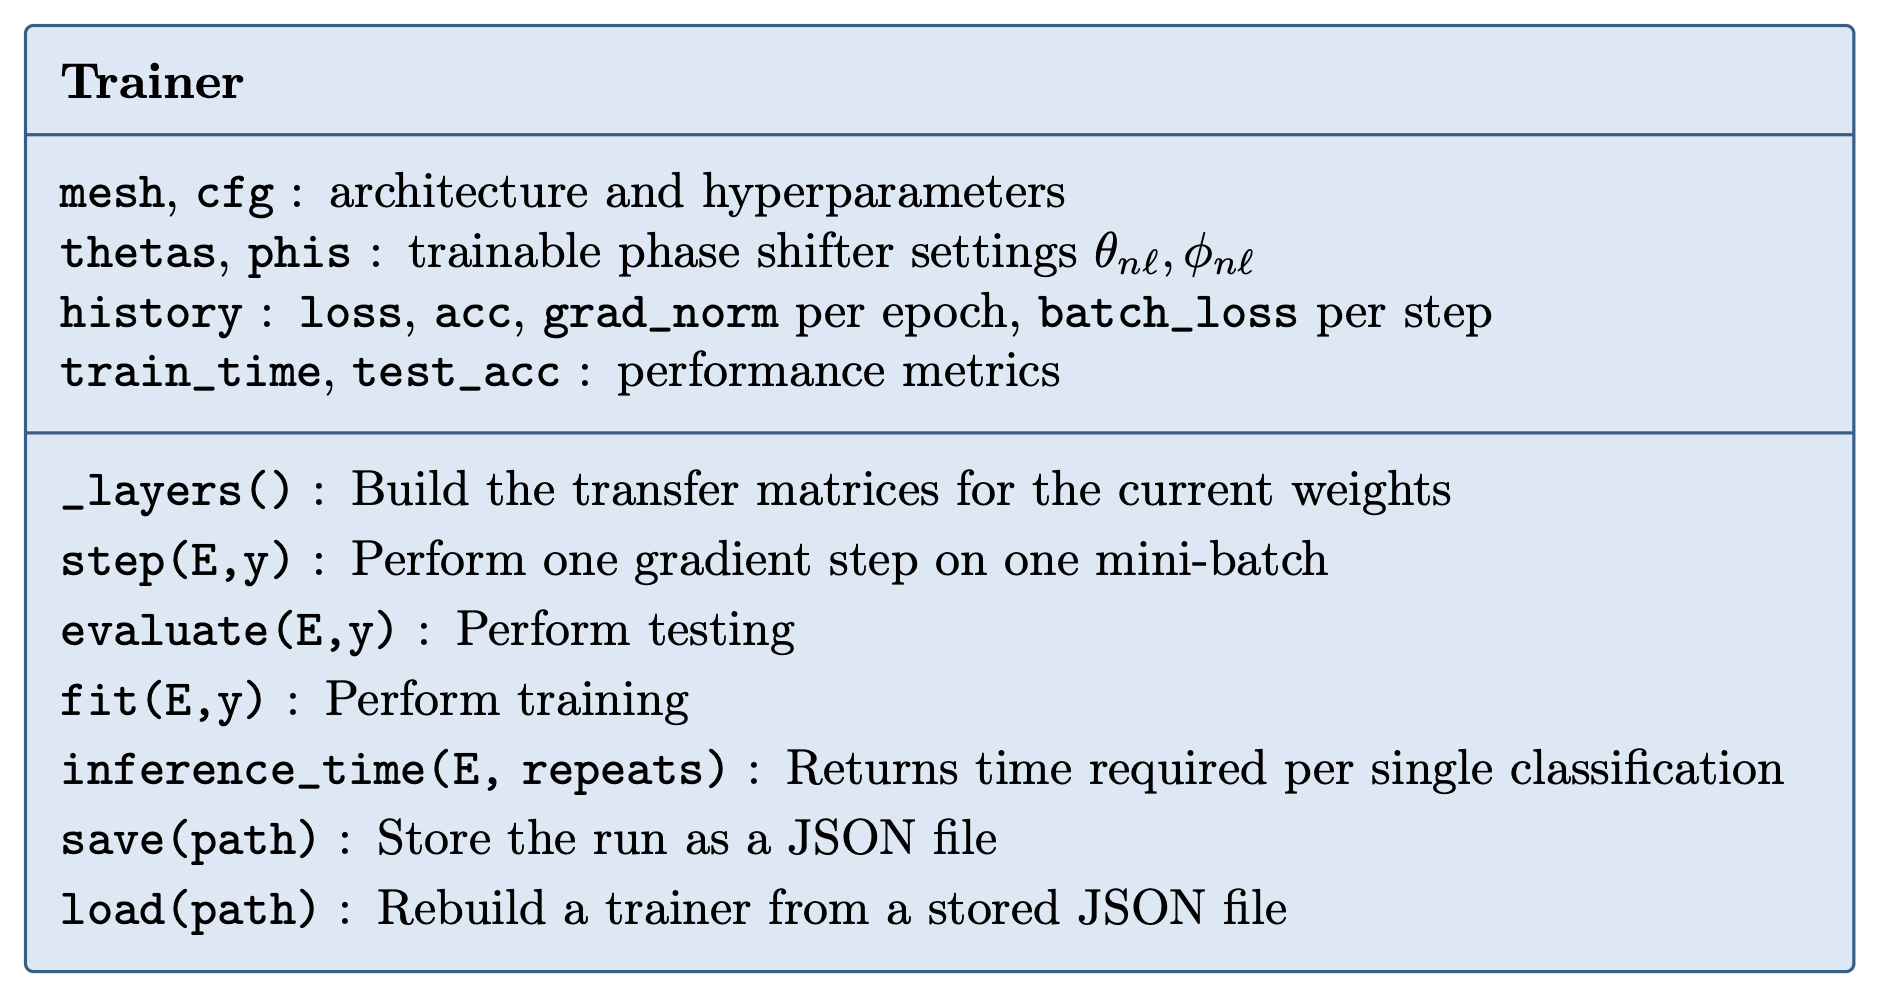
\includegraphics[width=0.7\linewidth]{images/main_classdiagram_trainer.png}
    \caption{Class diagram for \code{trainer} class from \code{trainer.py}.}
    \label{fig:class-trainer}
\end{figure}

\begin{figure}[H]
    \centering
    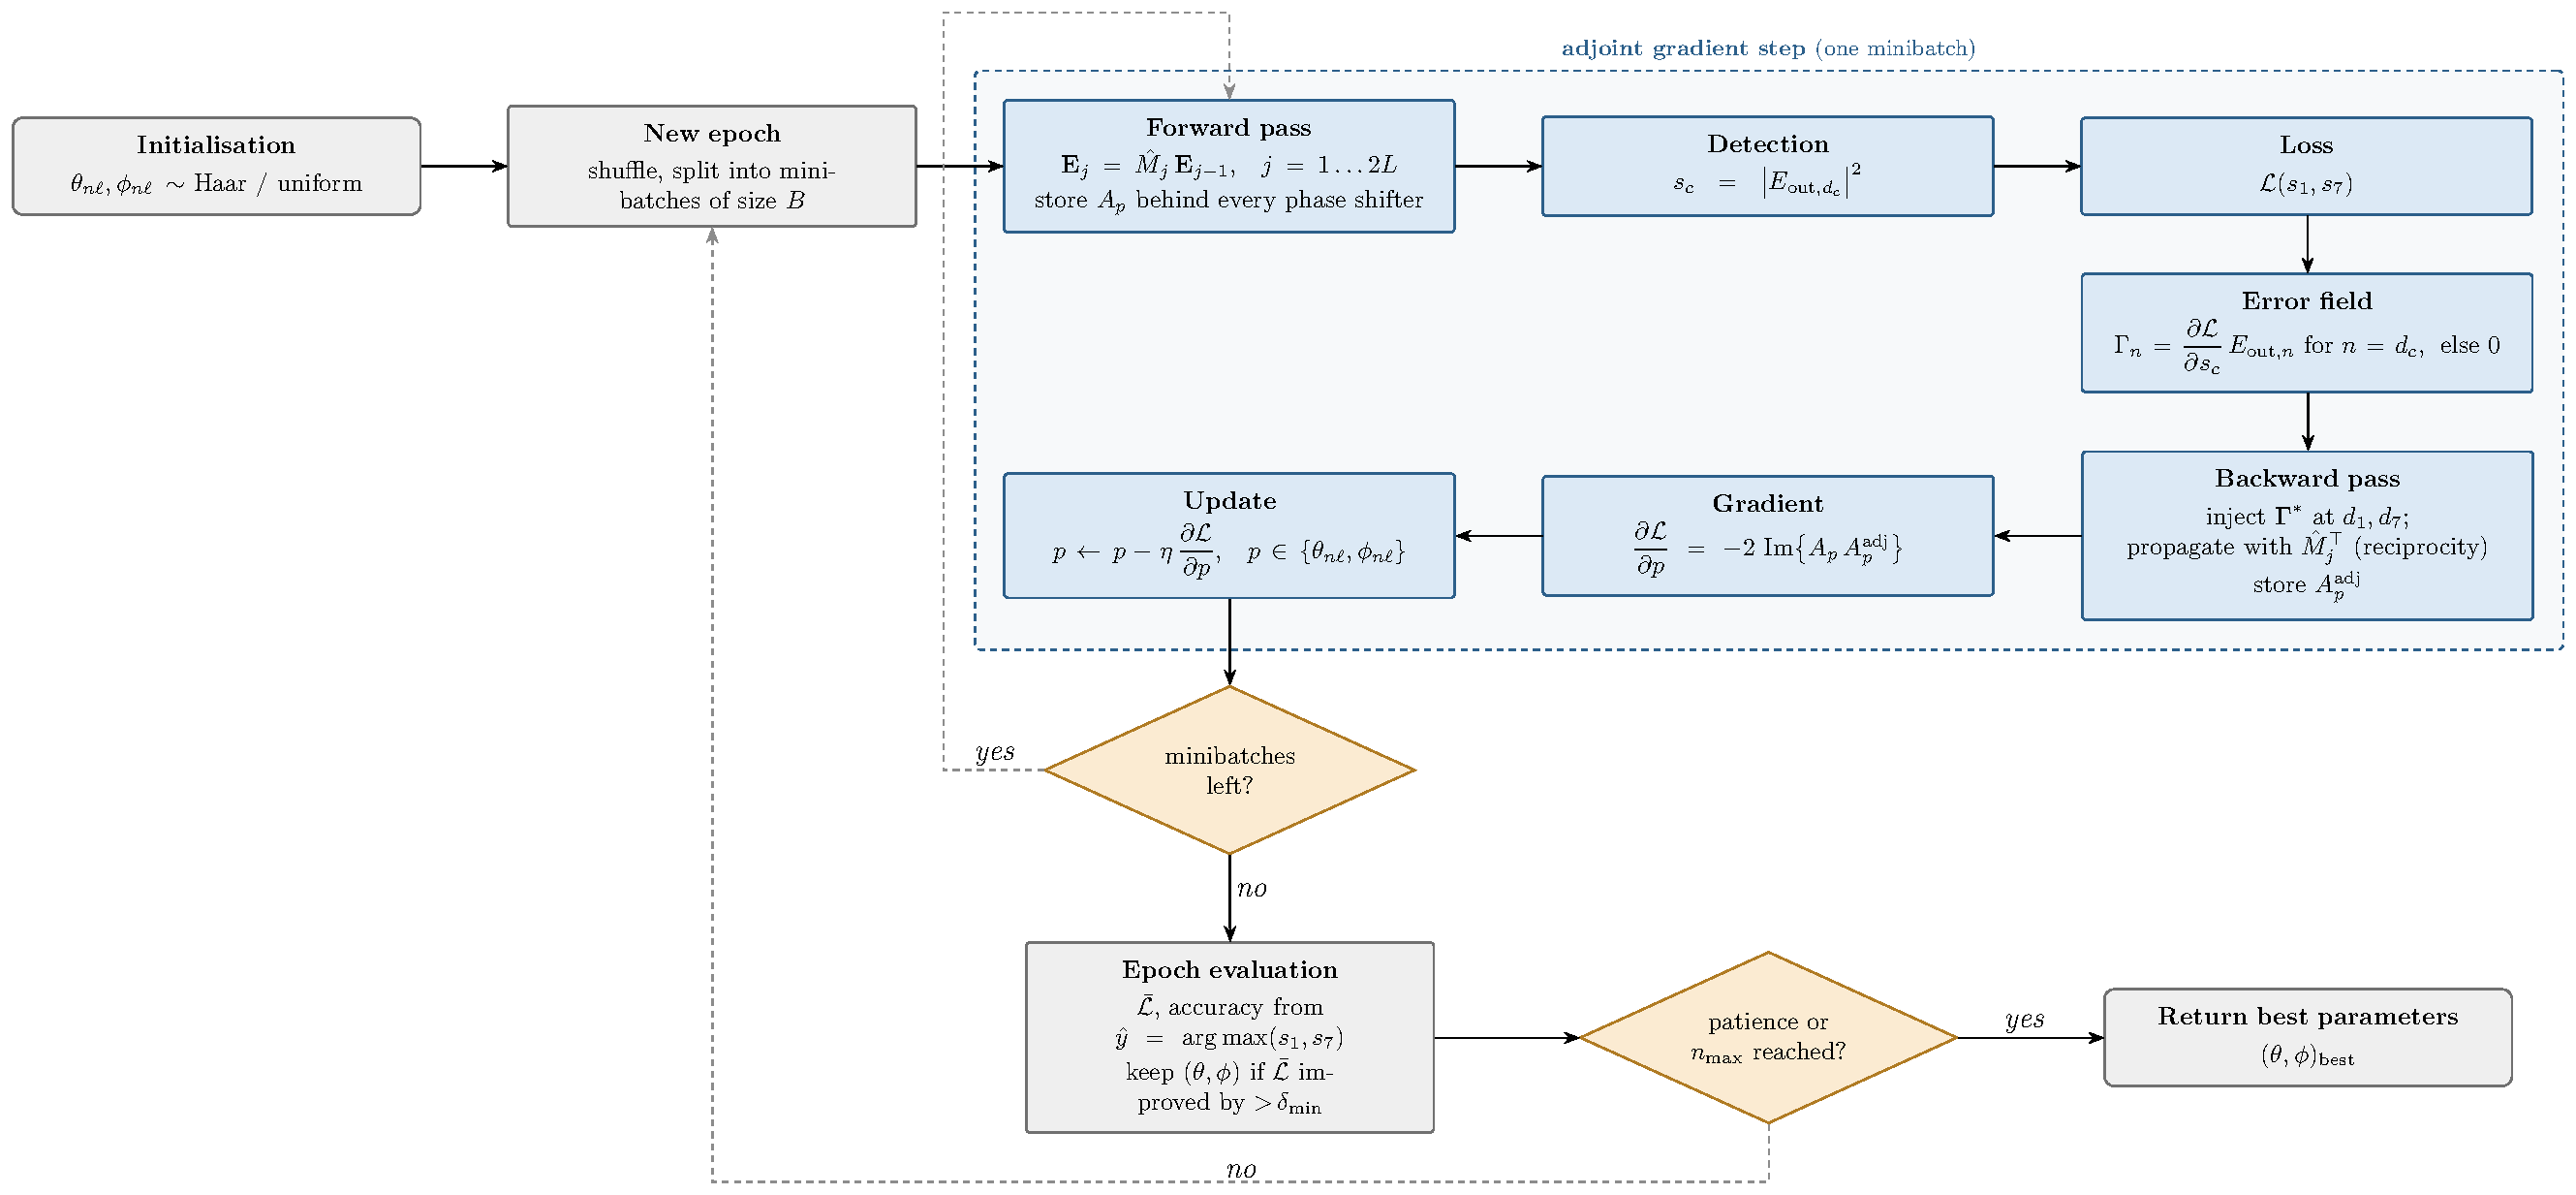
\includegraphics[width=\linewidth]{charts/trainer_algo_flowchart_horizontal.pdf}
    \caption{Flowchart of \code{fit}-algorithm in \code{trainer} class.}
    \label{fig:training_flow}
\end{figure}

%Conventional backpropagation operates on a known computational graph and requires the transpose of each weight matrix to be available as an explicit numerical object. In our system the weights are not numbers stored in memory but the phase settings of the \glspl{mzi} that are subject to drift.




\begin{figure}[H]
\centering
\begin{minted}
[
frame=none,
framesep=2mm,
baselinestretch=1.2,
bgcolor=codeyellow,
fontsize=\footnotesize,
linenos
]{python}
def gradient(fh, bh, plan):
    """Calculation of gradient for all values of theta and phi based on forward and backward
    propagating fields"""
    grad_th, grad_ph = [], []
    for l, (kind, ks) in enumerate(plan):
        gt = np.zeros(len(ks)); gp = np.zeros(len(ks))
        for i, k in enumerate(ks):
            # phase_shift applied to upper mode only
            gt[i] = -2*np.imag(np.sum(bh[2*l+1][k] * fh[2*l+1][k]))
            gp[i] = -2*np.imag(np.sum(bh[2*l+2][k] * fh[2*l+2][k]))
        grad_th.append(gt); grad_ph.append(gp)
    return grad_th, grad_ph
\end{minted}
\caption{Shortened excerpt from \code{processing.py} showing the function \code{gradient}.}\label{code:gradient}
\end{figure}

The loss function $\mathcal{L}(s_1, s_7)$ depends on the scores of the chosen detectors for the digits 1 ($s_1$) and 7 ($s_7$).
Two loss functions are implemented in \code{decoding.py}: mean square error (function \code{mse}) and softmax-cross-entropy (function \code{softmax\_ce}).
The mean squared error loss and its derivative with respect to the detector score can be defined as:
\begin{align*}
    \mathcal{L}_{\text{MSE}}(s_1, s_7) &= \sum_{c \in \{1,7\}} (s_c - t_c)^2 \text{ and }
    \frac{\partial \mathcal{L}_{\text{MSE}}}{\partial s_c} = 2(s_c - t_c).
\end{align*}

The softmax-cross-entropy loss and its derivative are given by:
\begin{align*}
    \mathcal{L}_{\text{CE}}(s_1, s_7) &= - \sum_{c \in \{1,7\}} t_c \log(p_c) \text{ and }
    \frac{\partial \mathcal{L}_{\text{CE}}}{\partial s_c} = p_c - t_c
    \text{ with }
    p_c = \frac{e^{s_c}}{e^{s_1} + e^{s_7}},
    %\label{eq:softmax}
\end{align*}
where $t$ is the target value.


\section{Training and performance evaluation} %2-3 pages
%
%- Performance metrics: training time, inference time
%- energy consumption
%
Over the whole project we stuck to the dataset of 1000 images of each class, split into 80\% training, 20\% testing using the function \code{get\_data} with the randomness seed ``1550'', our results are reproducible.
%One epoch has passed when each of the training images has been used once for the training.
The used parameters and results of the given tests can be retrieved from the JSON files in the results folder.

\subsection{Linear Regression}
As a baseline to compare our optical machine learning model against, a linear regression is performed.
The results of the linear regression with and without energy normalization and for different values of the image side-lengths ($m=[1,2,4,6,8,10,16,20,28]$) are compared. 
\begin{wrapfigure}{r}{7cm}
%\begin{figure}[H]
    \centering
    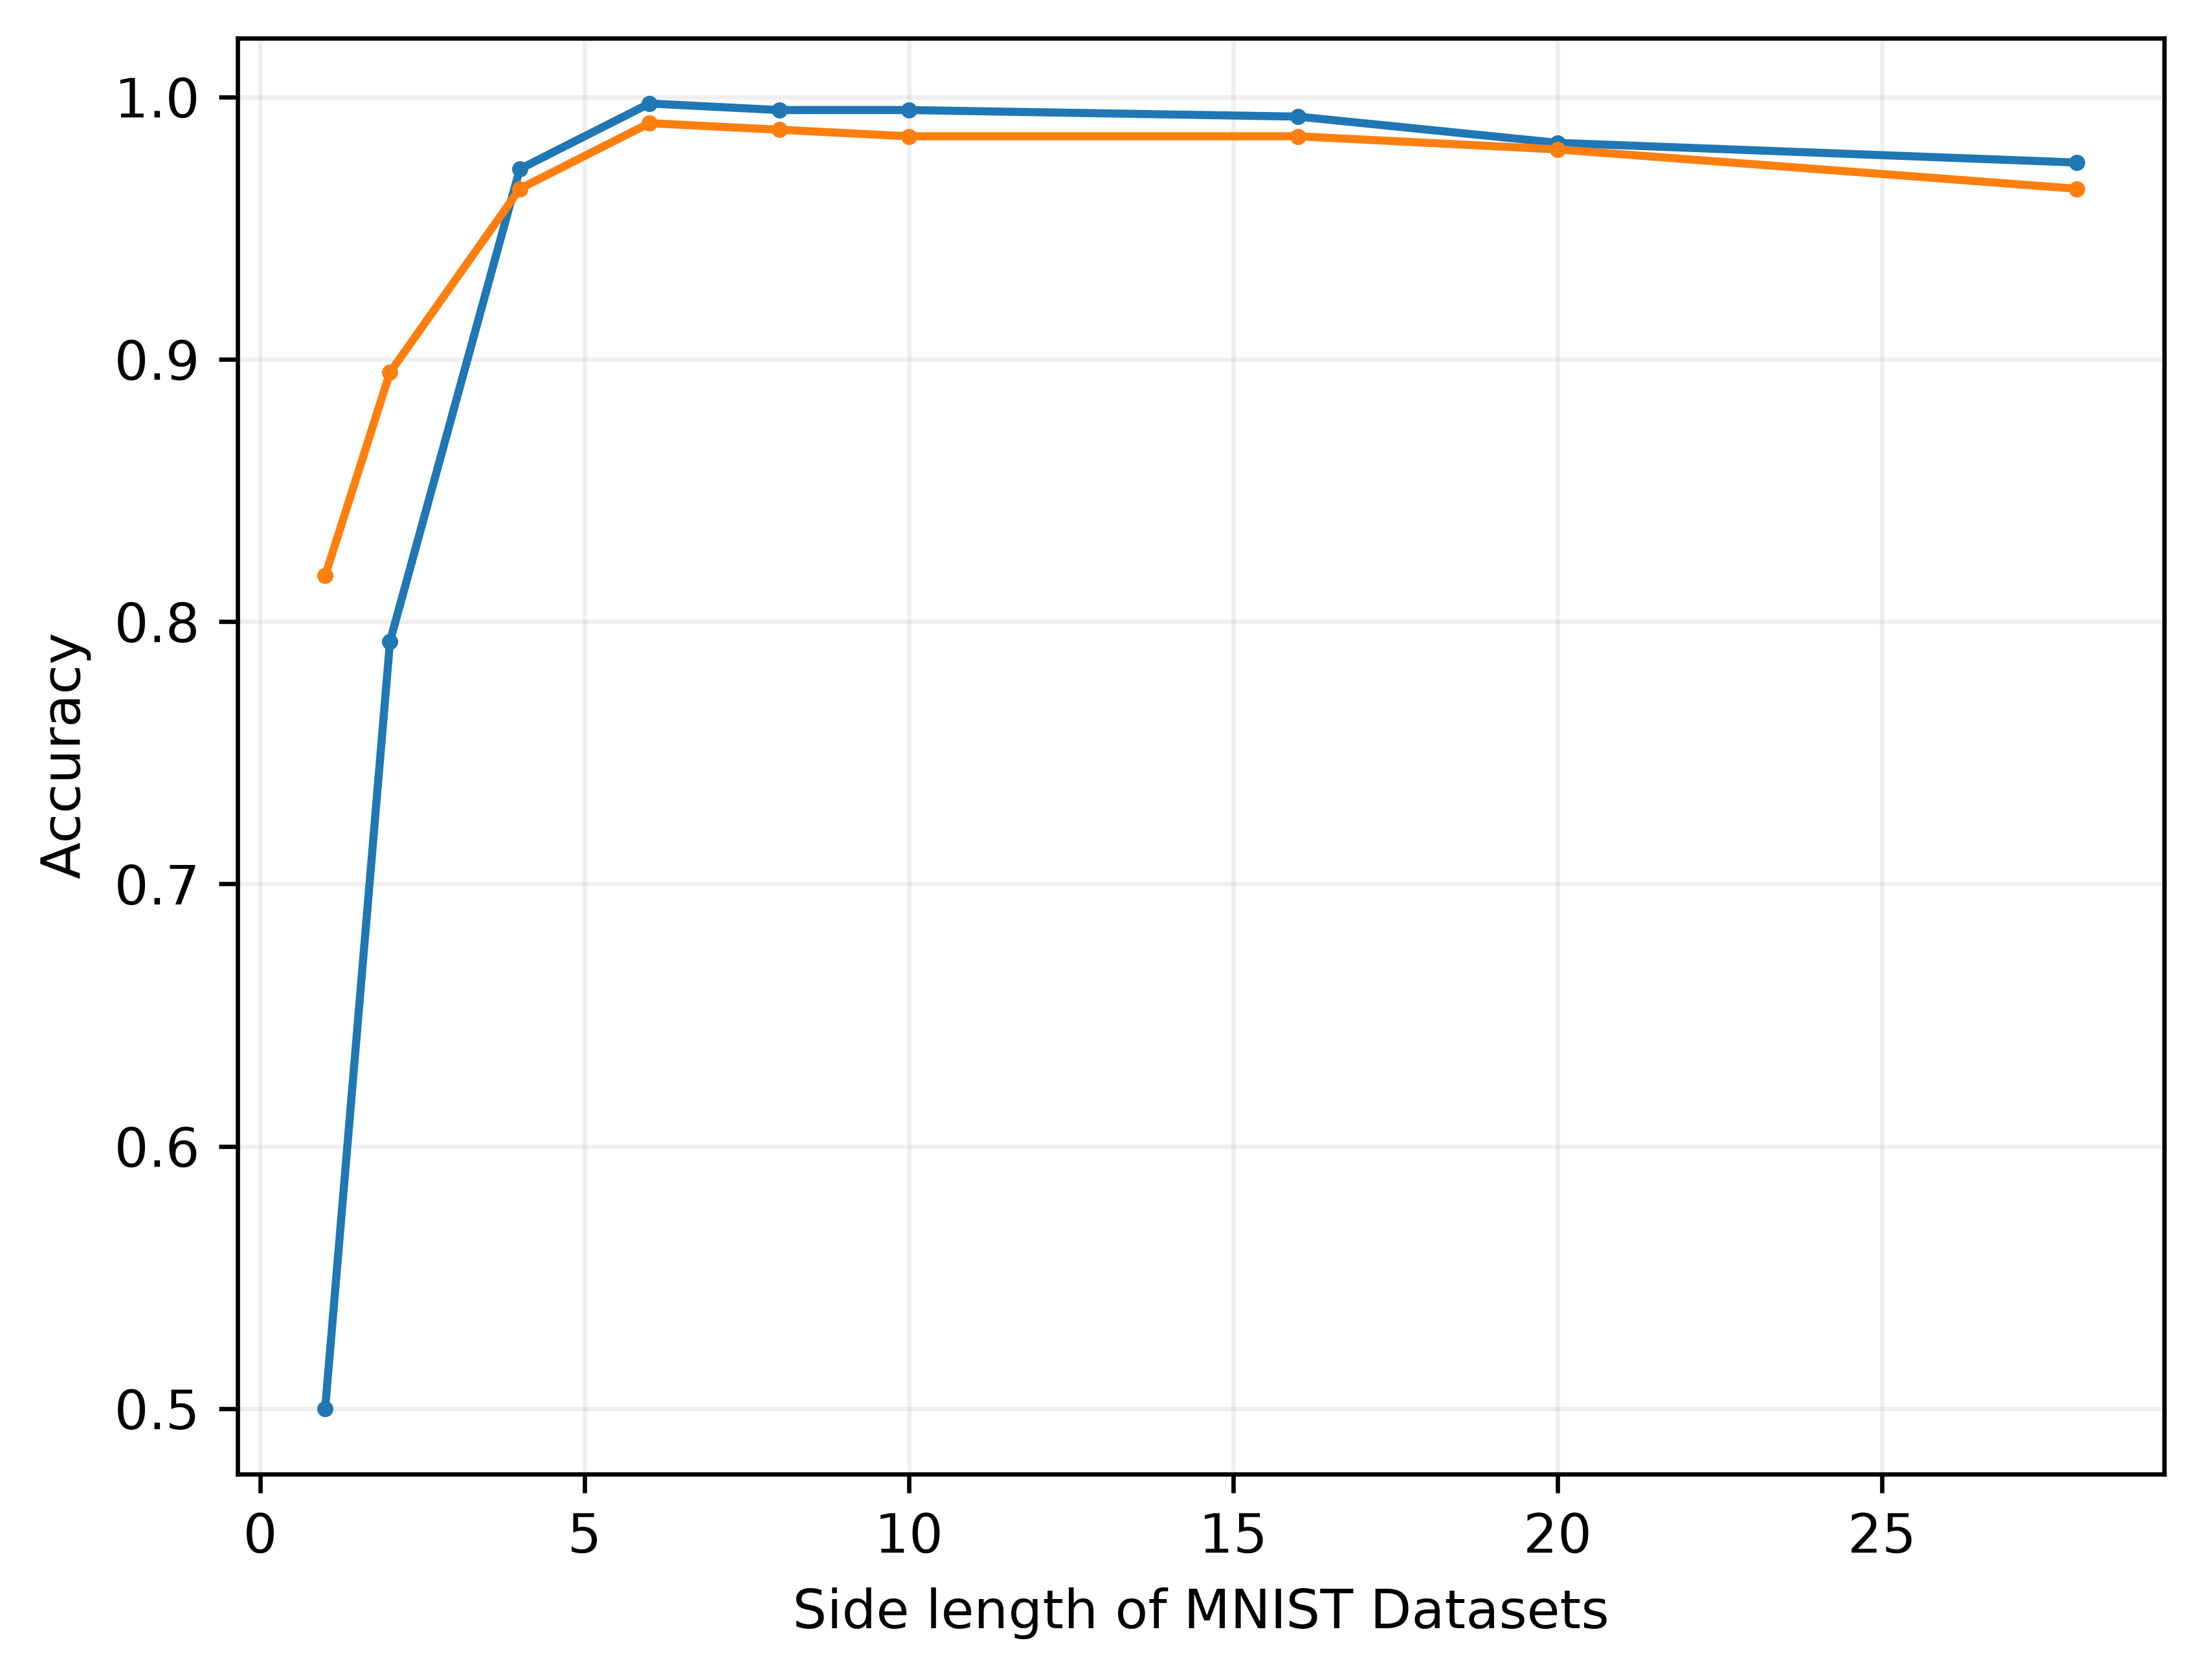
\includegraphics[width=0.9\linewidth]{evaluation/linear_regression/m_sweep_with_and_without_energy_normalization.png}
    \caption{Accuracy of the linear regression with (blue graph) and without (orange graph) energy normalization for different side lengths of the images.}
    \label{fig:linear_regression_m_sweep}
%\end{figure}
\end{wrapfigure}
A side-length of $m=6$\,px with energy normalization yields the highest testing accuracy with a value of 0.998.
For all m-values except $m=1$ and $m=2$, the energy normalization method yields better results.
The superior performance of the non-normalized case for these low m parameters is explained by the fact, that all of the information of the picture is contained in only one and 4 pixel respectively.
In this case, the model is basically trained on the ``used ink'' to draw the digit. This is also the reason why the energy-normalized mode performs better for larger m. If more information-carrying features are available, the information about overall energy in the system is more prone to generate confusion, for example due to a thicker written ``1''.
The high accuracy of the linear regression shows, that the given classifying problem is almost linearly separable. 

\subsection{Initialization of mesh's phase shift parameters and layer number}
\label{ssec:MeshInit}
The behavior and performance of our model is examined for the two different initialization methods.
In Figure \ref{fig:Mesh_Init_Random_and_Haar}, the intensities of an electric field at input port 50 are visualized.
It is visible that for the Haar initialization, the electric field reaches the edges of the mesh much faster than for the random initialization.
\begin{figure}[H]
    \centering
    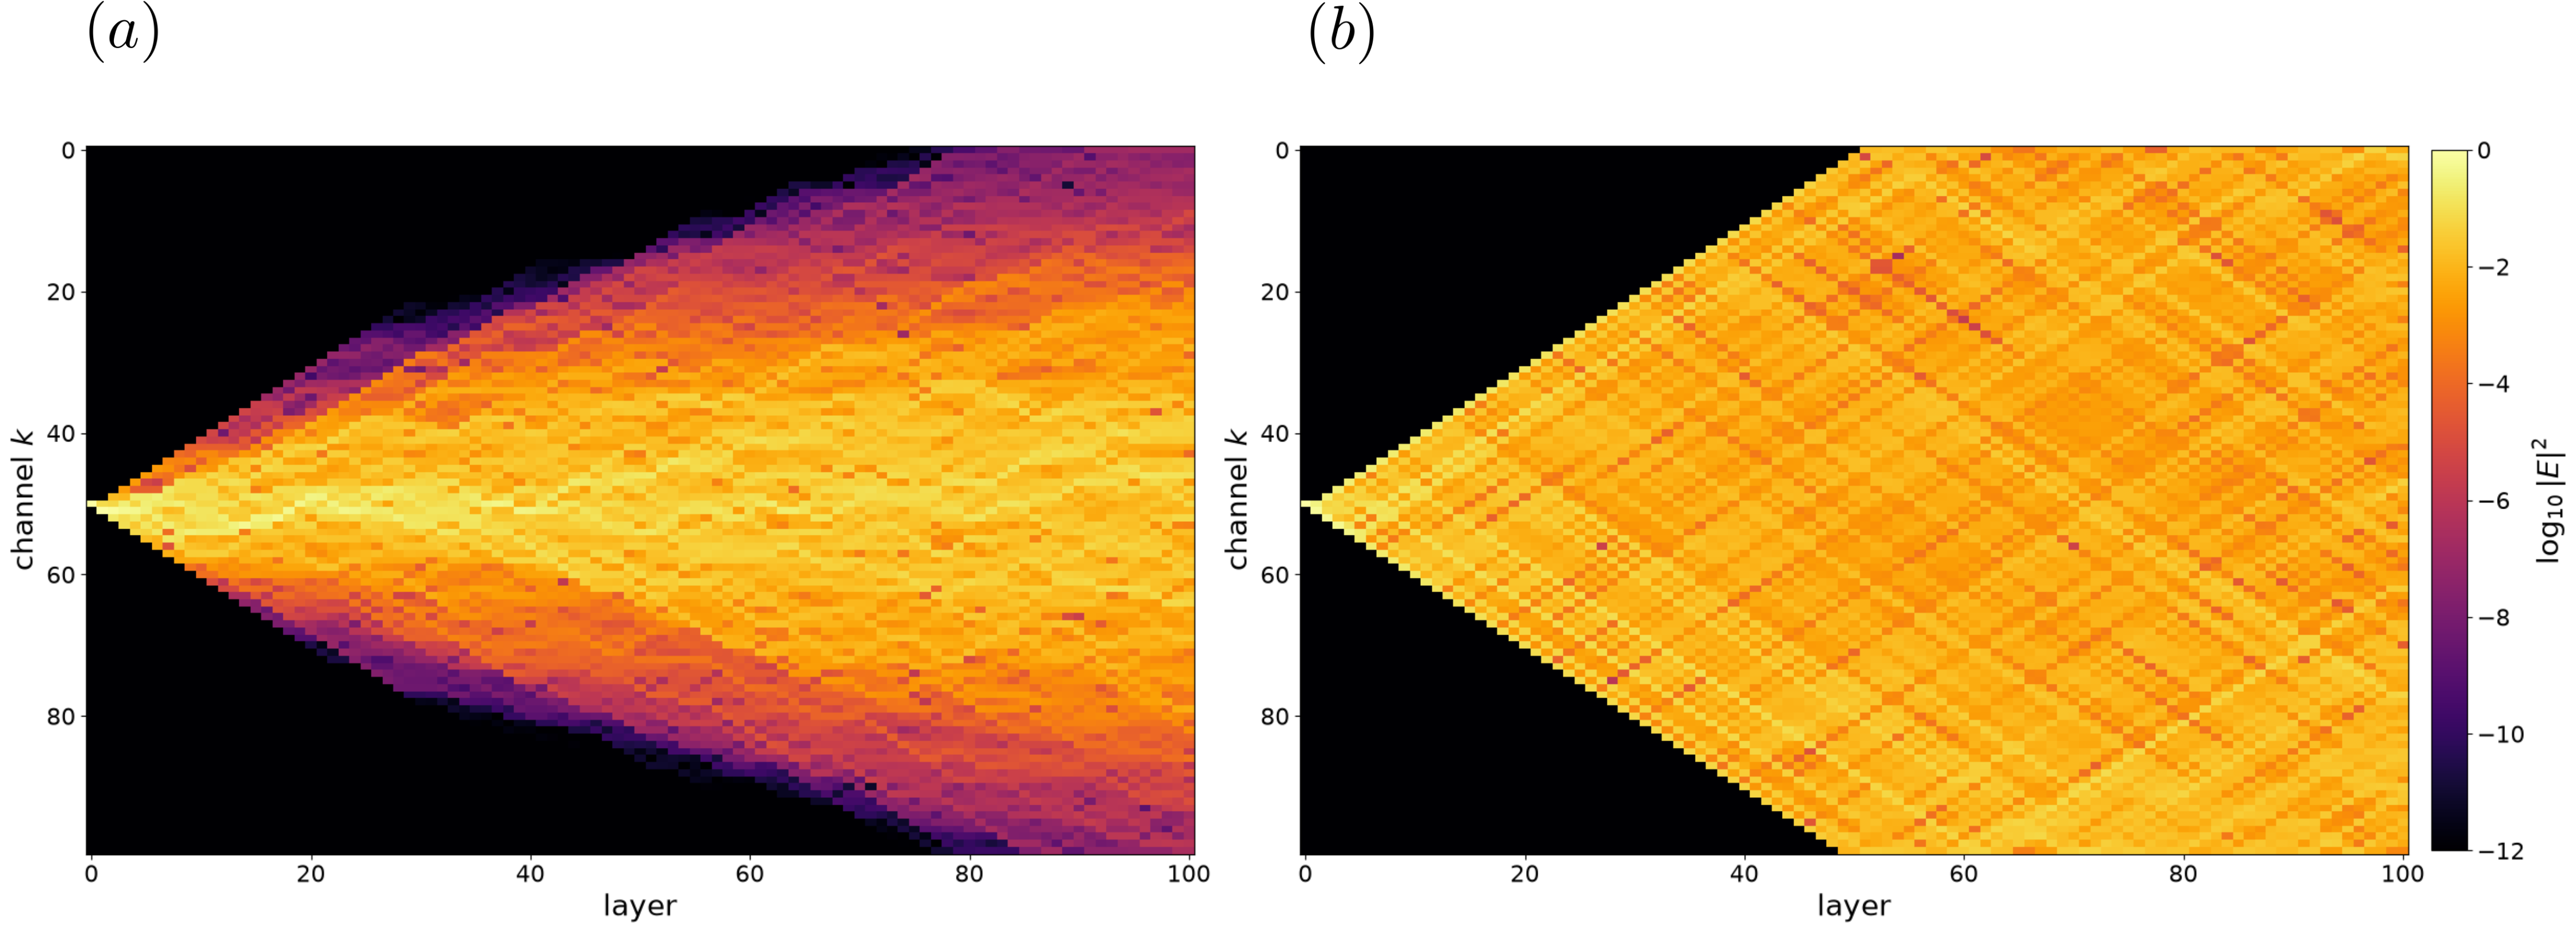
\includegraphics[width=0.8\linewidth]{evaluation/initialization/initComparisson.png}
    \caption{Intensity plot of a normalized electric field starting from channel 50. The mesh's parameters are initialized according to (a) uniform initialization, (b) Haar initialization for uniformly random global transfer matrices.}
    \label{fig:Mesh_Init_Random_and_Haar}
\end{figure}
The training and test results are shown in Figure \ref{fig:init_sweep}.
The training loss of the Haar initialization decreases faster than for the random initialization, leading to a faster convergence.
The random initialization reaches a training accuracy of 0.958 after 29 epochs or 355\,s. The testing accuracy is 0.980.
The Haar initialization reaches a training accuracy of 0.958 after 16 epochs or 185\,s, while the testing accuracy is 0.970.
\begin{figure}[H]
    \centering
    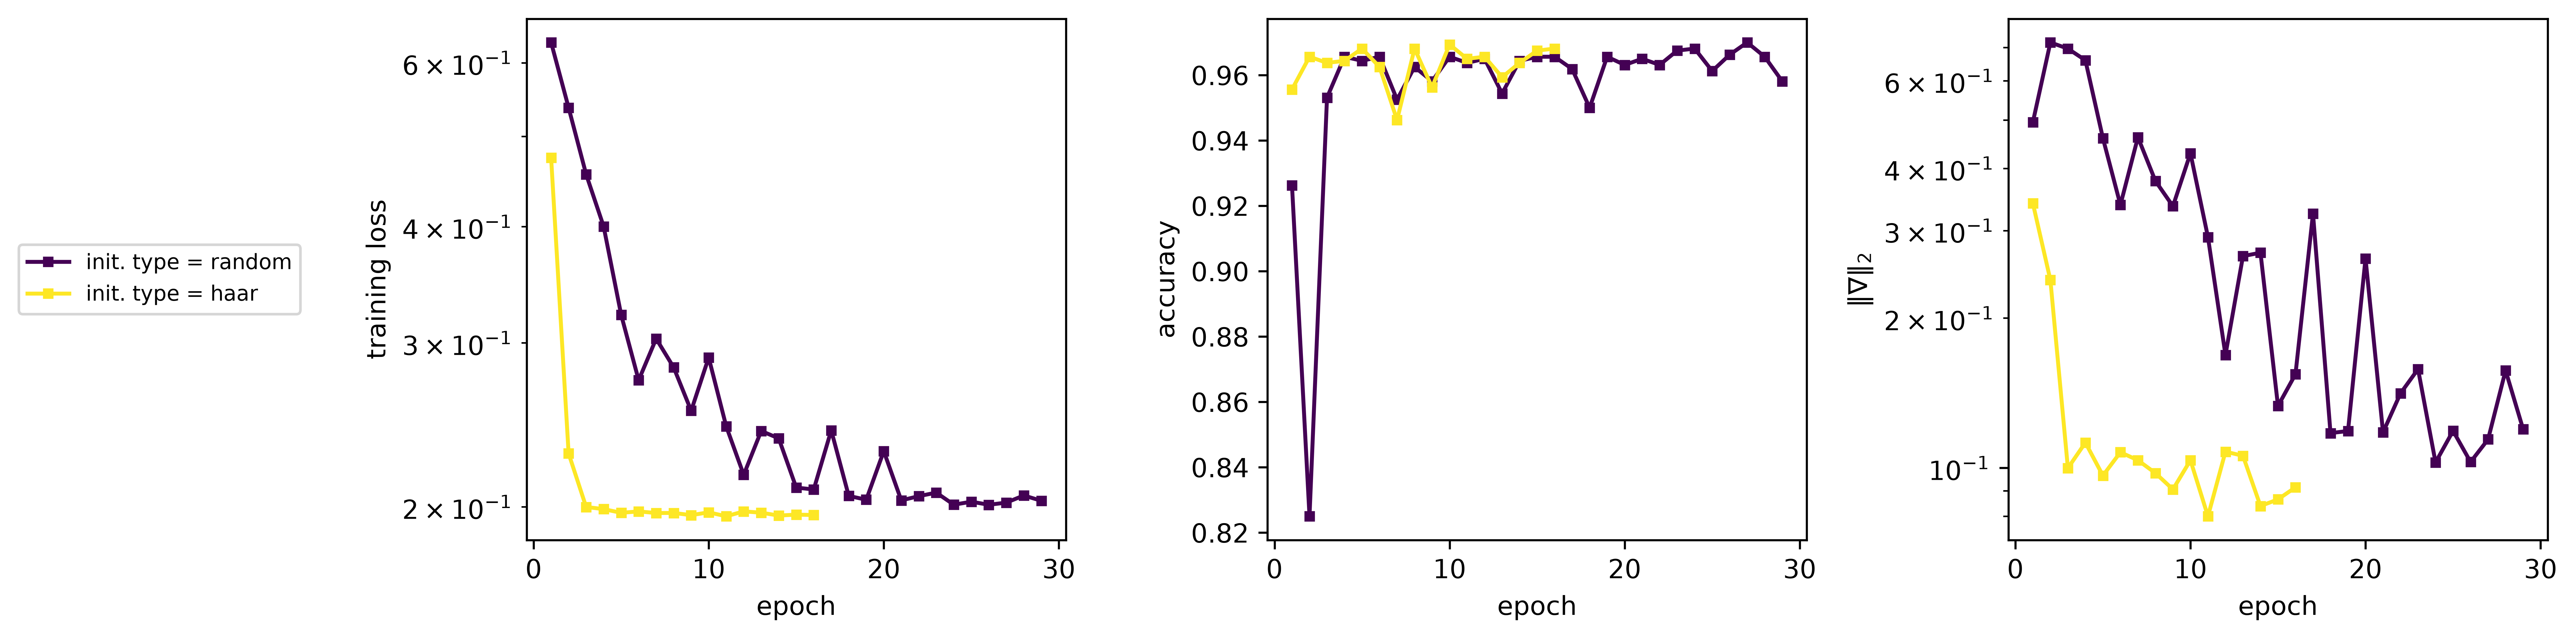
\includegraphics[width=\linewidth]{evaluation/initialization/plot_training_epoch.png}
    \caption{Training loss, training accuracy and normalized gradient for random and Haar initialization.}
    \label{fig:init_sweep}
\end{figure}
%init. type=random  epochs= 29 loss=0.20297  train acc=0.9581  test acc=0.9800  355s
%init. type=haar  epochs= 16 loss=0.19596  train acc=0.9681  test acc=0.9700  185s

%\subsection{Layer number}
To see impact of different \gls{mzi} meshes with respect to the layer number, we perform training over different values. Since the haar initialization promises for faster mixing of the signal inside the mesh over random initialization, we perform this training for both.
For Haar initialization, the performance of our model for different numbers of layers in the \gls{mzi} mesh is shown in Figure \ref{fig:layer_count_sweep}.
The training loss decreases most for the layer counts of 100 and 150, and least for the lowest layer count of 10. The training loss for 200 layers behaves similar to the next lower examined layer counts, but is slightly higher.
The training accuracy is highest for the layer counts of 100, 150 and 200.
For the random initialization, see Figure \ref{fig:layer_count_sweep_random_init}, the relative performance is equivalent with higher layer counts converging faster and yielding higher accuracies. Compared to the previous initialization however, the slower convergence becomes clearly visible for all layer sizes. Also the maximum achieved testing accuracy with 0.968 is subordinate to the value of 0.975 of the Haar initialization.
Since less layers mean a less complex physical setup and consequently less losses, the Haar initialization allows a smaller setup.

\begin{figure}[H]
    \centering
    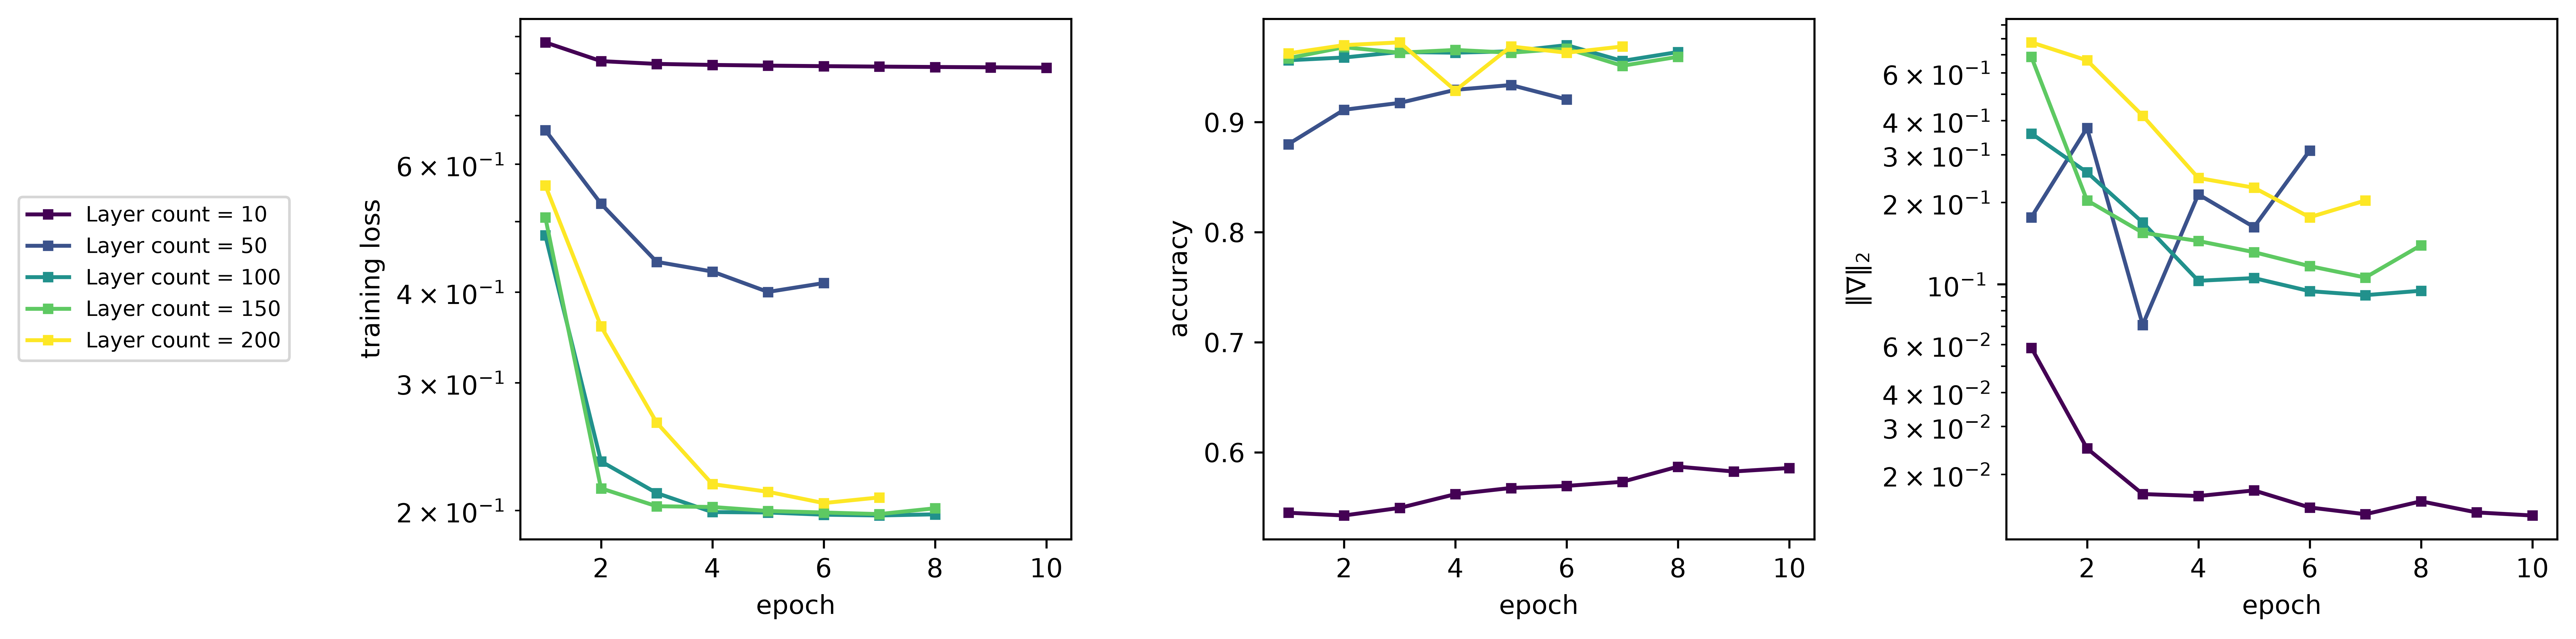
\includegraphics[width=1\linewidth]{evaluation/layer_count/plot_training_epoch.png}
    \caption{Training loss, training accuracy and normalized gradient for different numbers of layers with Haar initialization.}
    \label{fig:layer_count_sweep}
\end{figure}

\begin{figure}[H]
    \centering
    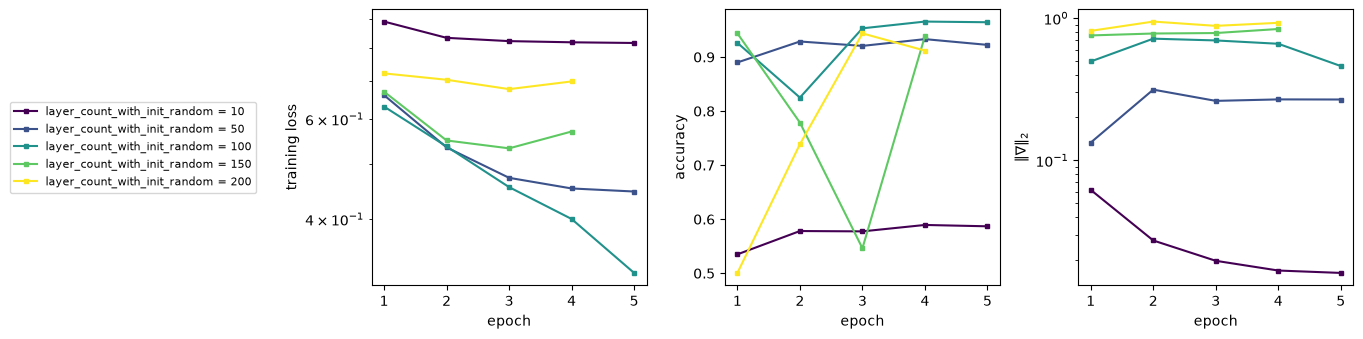
\includegraphics[width=1\linewidth]{evaluation/layer_count/plot_training_epoch_random_init.png}
    \caption{Training loss, training accuracy and normalized gradient for different numbers of layers with random initialization.}
    \label{fig:layer_count_sweep_random_init}
\end{figure}


\subsection{Learning rate analysis}
Sweeping over different learning rates is performed to see the effect on the convergence speed and the achieved accuracy.
We limit the runtime by using a patience value of 5 and a \code{min\_delta=1e-4}. Therefore, we make sure not to waste training time when no further improvement or no convergence at all is possible.
We run it over three different batch sizes (256, 64 and 4). We begin by using 64 to find the best performing learning rate (see Fig. \ref{fig:learning_rate_medium_batch_sweep}) and use 256 and 4 (see appendix \ref{appendix:graph-learningrate}) to see how this optimal learning rate differs based on batch sizes.

The highest learning rates converge fast but reach only a low training accuracy.
It is clearly visible how lower learning rates lead to a slower but more stable convergence. 
This behavior is confirmed for all three tested batch sizes.
Based on the results, a reasonable trade-off seems to be reached for learning rates of 1.0 to 1.7.
\begin{figure}[H]
    \centering
    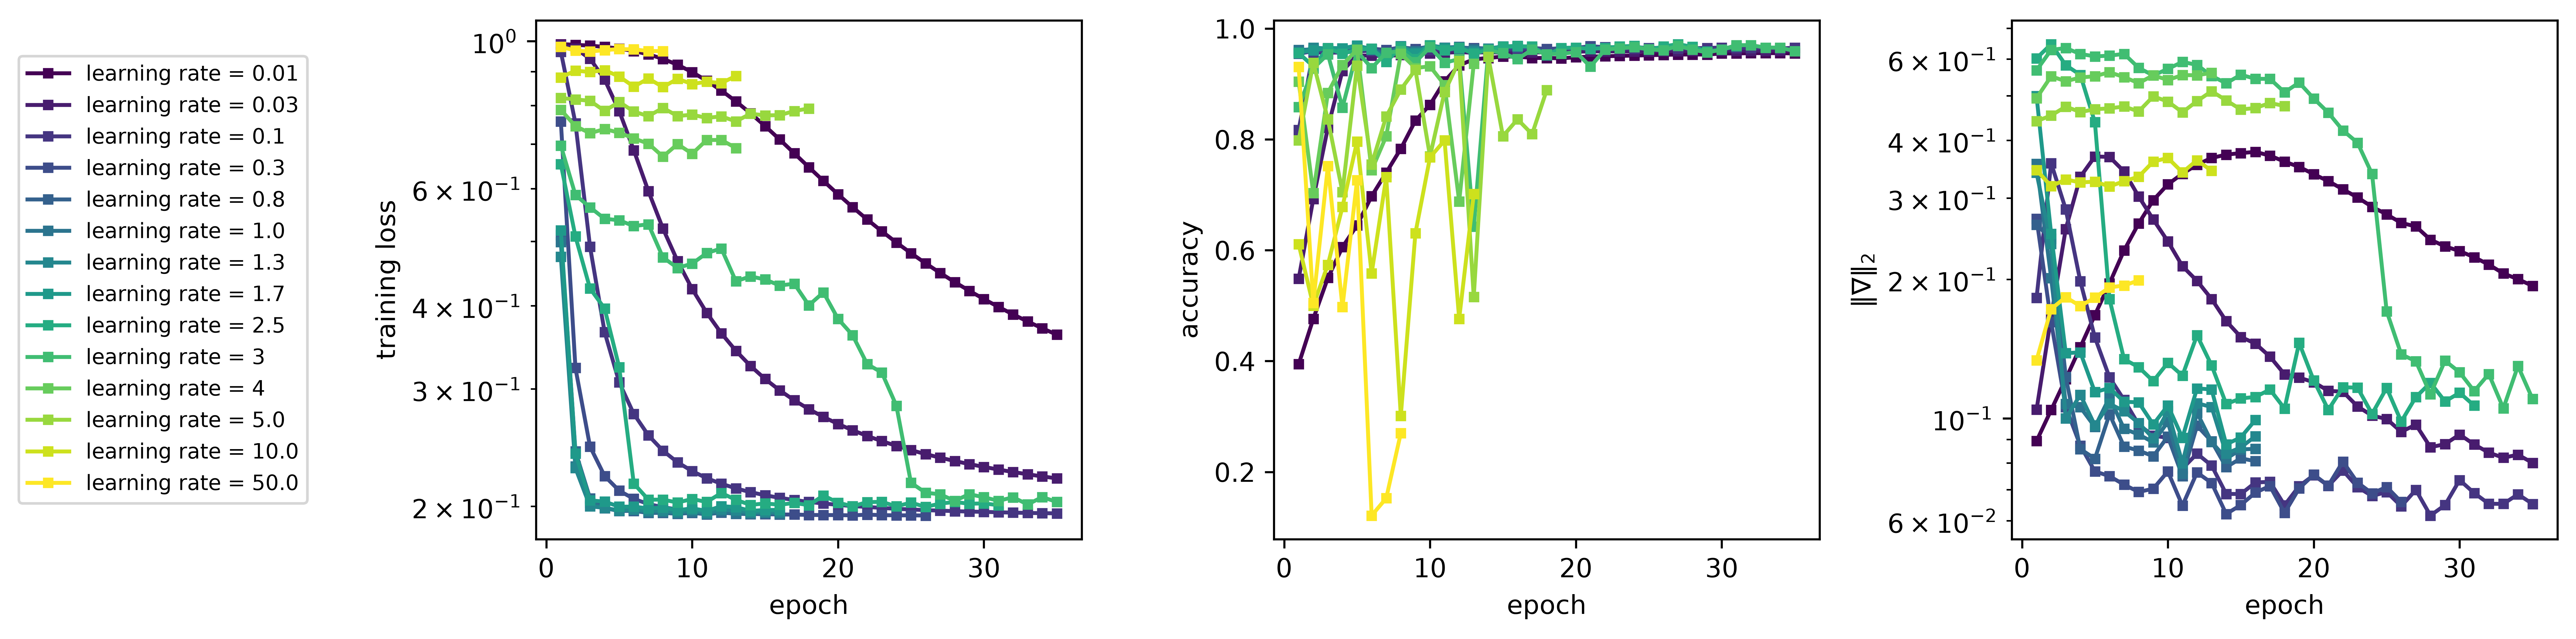
\includegraphics[width=1\linewidth]{evaluation/learning_rate/64_plot_training_epoch.png}
    \caption{Training loss, training accuracy and normalized gradient for different learning rates for a batch size of 64.}
    \label{fig:learning_rate_medium_batch_sweep}
\end{figure}

%Interestingly, the gradient norm for the lowest learning rate is increasing first, until reaching a maximum and the decreasing. 
%Hier außerdem ganz interessant, dass man bei der gradienten Norm sieht, wie die langsame Kurve wohl eine Verringerung des losses erreicht, in dem sie zunächst durch die loss landschaft wandert, wo die gesamte gradienten norm (da gibts so ein Wort) erstmal zunimmt, aber da halt die "wichtigeren" Parameter dann wohl zu einer verringerung des Losses führen.

\subsection{Side length analysis (down-sampling)}
The performance for different side lengths of the down-sampled MNIST images was investigated for side lengths of $m=[6,8,10,14,18,22]$.
The detector positions are scaled with the side length and placed at one third and two thirds of the total number of output ports.
The results are shown in Table \ref{tab:side-length} (see also Figs. in appendix \ref{appendix:graph-m}).
The achieved training loss, training accuracy and normalized gradient are similar over all tested side lengths, except for the lowest side length, which shows the worst training accuracy.
When observing the reached accuracies as a function of the necessary time, it is obvious, that for our simulation higher side lengths lead to far longer computation times while not offering performance improvements after a side length of 14.
It should ne noted, that for the physical system more parameters should not lead to an increased training time because all adjustments and measurements can happen in parallel.
% "max_epochs": 10,"patience": 3,"min_delta": 0.001,
\begin{table}[H]
    \centering
    \caption{Training time and achieved testing accuracy for the different side lengths of the down-sampled MNIST images.}
    \begin{tabular}{|c|c|c|}
    \hline
    Side length & Training time in s & Testing accuracy\\
    \hline
        6 & 10 & 0.933\\
        8 & 62 & 0.960\\
        10 & 103 & 0.978\\
        14 & 519 & 0.988\\
        18 & 1398 & 0.978\\
        22 & 3307 &0.980\\
    \hline
    \end{tabular}
    \label{tab:side-length}
\end{table}

\subsection{Batch size analysis}
The influence of the batch size is evaluated in Table \ref{tab:batch-size} (see also Figs. in appendix \ref{appendix:graph-batchsize}).
For this test a learning rate of 0.1, a patience of 3 epochs and maximum number of 10 epochs were chosen.
The highest testing accuracy of 0.978 is achieved for a batch size of 1.
At the same time, the computation time increases with lower batch sizes due to the increased number of gradient updating steps. Here, a similar behavior of the physical system would be expected.
Overall, it is possible to already reach high testing accuracies after short training times using a larger batch size. For all batch sizes a similar training accuracy is achieved.
\begin{table}[H]
    \centering
    \caption{Training time and achieved testing accuracy for the different batch sizes.}
    \begin{tabular}{|c|c|c|}
    \hline
    Batch size & Training time in s & Testing accuracy\\
    \hline
        1 & 2801 & 0.978\\
        2 & 501 & 0.965\\
        4 & 785 & 0.945\\
        8 & 425 & 0.968\\
        16 & 207 & 0.973\\
        32 & 166 & 0.970\\
        64 & 87 & 0.970\\
        128 & 56 & 0.965\\
        256 & 40 & 0.963\\
        512 & 32 & 0.973\\
    \hline
    \end{tabular}
    \label{tab:batch-size}
\end{table}

\subsection{Loss function comparison}
The influence on the performance of the loss function was investigated by comparing the mean square error loss function and the softmax cross-entropy loss function (see Fig. \ref{fig:loss_func_comparison}).
For the loss functions a testing accuracy of 0.970 and 0.968 is reached respectively, therefore both seem to perform similarly well.
The batch loss shows the loss for each mini-batch within one epoch.
The difference of the absolute loss between the functions is due to the difference between their ``target value''. 
The mean square error tries to minimize the intensity in all detectors but the target one to zero, while the softmax function does not.
Thus, it is not possible to compare the functions based on their absolute loss.
\begin{figure}[H]
    \centering
    
\includegraphics[width=1\linewidth]{evaluation/loss_function/plot_training.png}
    \caption{Batch loss, training loss, training accuracy and gradient for the two loss functions.}
    \label{fig:loss_func_comparison}
\end{figure}

\subsection{Hyperparameter theta\_enc (in phase encoding)}
\label{sec:AmplitudeEncoding}
The influence of the encoding hyperparameter \code{theta\_enc} is examined for the phase encoding (see Tab. \ref{tab:phase_enc}, see also Fig. in appendix \ref{appendix:graph-thetaphase}).
It does not have to be considered for the amplitude encoding because it is a factor which would increase the value of all inputs in the same way. In phase encoding however, this parameter scales the phase according to $E_j=\exp{(i \cdot \theta \cdot \pi \cdot V_j)}$.
%\begin{align*}
%    E_j=\exp{(i \cdot \theta \cdot \pi \cdot V_j)}.
%\end{align*}
By this we introduce another non-linearity that is relevant even with normalized energy.
For low values of \code{theta\_enc}, the training takes comparatively long, while reaching a low testing accuracy.
The highest testing accuracy of 0.983 is reached for \code{theta\_enc} of 0.750.
\begin{table}[H]
    \centering
    \caption{Relevant results for different hyperparameters \code{theta\_enc} for phase encoding.}
    \begin{tabular}{|c|c|c|c|c|}
    \hline
    Theta\_enc & Epochs & Training accuracy & Testing accuracy & Training time in s\\
    \hline
        0.25  &  8  &  0.878 & 0.500 & 102\\
        0.5 & 8 & 0.933 & 0.583 & 101\\
        0.75 & 6 & 0.946 & 0.983 & 88\\
        1.0 & 6&  0.968 & 0.980 & 73\\
        1.5 & 6&  0.970 & 0.978 & 73\\
        2.0  &5 & 0.973 & 0.953 & 69\\
    \hline
    \end{tabular}
    \label{tab:phase_enc}
\end{table}

\subsection{Our best model}
We reached our highest testing accuracy of 0.990, meaning only 4 of the 400 test samples were misclassified. 
The used parameters are phase encoding with \code{theta\_enc}=0.75, energy-normalization, $m=14$, mean square error loss, a learning rate of 1.0, a batch size of 64 and Haar initialization. 
The training stopped after 5 epochs due to reaching the convergence criteria based on a patience of 1 and \code{min\_delta}=0.0001.
Switching from random to Haar initialization and from amplitude to phase encoding appears to offer significant improvements.
Here, the training took 129\,s, while the inference time is only 7.86\,ms per sample.
%Epoch 5.00/10 | Loss: 0.2141:  50%|█████     | 125/250.0 [02:08<02:08,  1.03s/it]
%validation acc 0.9669 | test acc 0.9900 | 5 epochs, 128.5s
%inference: 7.86 ms/sample

% mention training and inference time here!!!!!

\subsection{Outlook}
Further tests, that could be performed using our implemented model, would be a variation of the detector positions, a study of the optimal parameters for other mesh architectures as well as a resistance analysis studying the influence of losses in the beam splitters and fibers.
While an expansion to more digits would be interesting, minor changes to some of the implemented functions would be necessary.





\section{Discussion and critical analysis} %1-2 pages
\subsection{Bias-variance trade-off analysis}
To examine our optical system, a bias-variance trade-off analysis is performed considering the results of the training.
The bias is related to underfitting and describes errors which are caused when a model is too simplistic, while the variance refers to overfitting and a too high complexity.

The use of a \gls{mzi} mesh limits our model to unitary matrices. 
Additionally, the only non-linearity present in our model is the detection as intensity. This could be changed by adding a non-linearity between layers (\gls{onu}).
Thermal and detector noise, imperfections in the fabrication of the chip and losses at the beam splitters and fibers might lead to additional errors contributing to the variance.
Furthermore, the number of layers limits the number of adjustable parameters. Therefore, a low number of layers will contribute to the bias, while a high number of layers contributes to the variance.
A similar argument can be made for the side length of the images. When too few pixels are used, relevant information is lost, while for too many pixels, the model trains on ``noise''. Therefore, the best accuracy can be reached when a reasonable trade-off between these aspects is found, as demonstrated in the previous section on our best-performing model.

\subsection{Implementation challenges}
The main challenge of the computational as well as physical implementation of this model is the estimation of the gradient. %The solution is well-documented in the literature.
To calculate the gradient, the time-reversal interference method is used \cite{hughesTrainingPhotonicNeural2018}.
In the physical implementation, the non-measurability of the electric fields and the consequent need to use the measurable intensities for the computation lead to further complexity.

In our computational implementation the high runtime can pose a challenge. The main contribution appears to be the gradient update.
It would be possible to reduce the runtime by exchanging the element-wise loop-based update for a matrix-based solution.
Furthermore, the function \code{layer\_matrices\_separate} which constructs the matrices might be optimized by taking advantage of the sparse block-based structure and exchanging the appending to a list to the storage in a numpy array.
%- 153 ms für den Matrixbau sind unverhältnismäßig —  erzeugt 200 volle 100×100-Matrizen, obwohl jede nur 2×2-Blöcke auf der Diagonale trägt. Auch die Multiplikation M @ E rechnet dann O(N$^2$B) statt der eigentlich nötigen O(NB).
%Das ließe sich um etwa den Faktor 50 beschleunigen, indem man die Blockstruktur ausnutzt statt volle Matrizen zu bauen.

The chosen number of samples of 2000 seems to be rather low. It might make sense to repeat the tests with more samples to ensure that the dataset shows a realistic representation of the variance of the written digits.
%Unbedingt auf "Stichprobenrauschen" eingehen, das bei dieser Datengröße schon viel ausmacht (weiß auch nicht wie genau ich da quantitativ werden würde)

%Erkläre den Unterschied in der Modellklasse. Die lineare Baseline zeigt, wie viel schon linear geht; dein Mesh zeigt, dass ein energieerhaltendes optisches System dieselbe Aufgabe physikalisch realisierbar löst — was der eigentliche Punkt eines optischen Computers ist. (lineare regression hat viel mehr freiheiten bei der Matrix, wir haben zwar mehr Parameter aber die Matrix muss unitär sein (energieerhaltung), deshalb hat es unser System "schwerer"


\subsection{Estimated energy consumption}
The consumed energy of the physical model depends on the laser, the control of the encoding, the control of the phase shifters, the detectors and the computing for the encoding and decoding.
Compared to the energy consumption of the laser and an assumed electro-optic control of the phase shifters, the other contributions are probably negligible.
While the energy consumption of the electro-optic modulators should be constant over time, the energy consumption of the laser depends on the time that the laser is turned on, and therefore the time required for one processing of one sample times the number of processing steps within the training.
After training of the model, for the testing only one forward propagation of the light is necessary.


\newpage

\section{Conclusion} 
%1/2 page
% Summary of best classification results achieved (requirement f)
%- Key insights and lessons learned
%- Suggestions for future improvements
We achieved the best classification result based on testing accuracy for the linear regression, where we calculated a testing accuracy of 0.998 for m=6 and energy normalization of the image vectors.
For our model, we achieved the highest testing accuracy of 0.990 after 5 epochs for the use of phase encoding with \code{theta\_enc}=0.75, energy-normalization, $m=14$, mean square error loss, a learning rate of 1.0, a batch size of 64 and Haar initialization, a patience of 1 and \code{min\_delta}=0.0001.

For the binary classification of digits ``1'' and ``7'', the linear regression outperformed our model, as this problem appears to be linearly separable.
If the classification was expanded to include more digits or when two other digits were chosen, these results might change.
Nevertheless, using the optical system it was possible to reach a testing accuracy close to the result of the linear regression.

As was shown, the model's performance can be improved by optimizing the hyperparameters, providing insights that might be transferred to the physical implementation.
The Haar initialization outperformed the random initialization of parameters.
The performance does not improve infinitely with increasing layer count and side length of the images, but it reaches an optimum for certain parameters. Before fabricating a physical chip, it is important to optimize these parameters.%Therefore a physical model of the best parameters could be built.

In comparison to the physical implementation, in the simulation it was possible to ``measure'' the electrical field at each position, simplifying the method. In a physical system only the intensities would be accessible. Thus the training method becomes more complicated, as the ``time-reversal interference method'' should be applied.
It would be possible to model this measurement protocol as well.
The most time-consuming step of our model is the gradient update. But the training does not seem to scale with the number of parameters, enabling the simulation of large models.
We would expect to observe the same behavior for the physical model.

As an outlook, it would be interesting to expand the model to more digits and to include losses and noise to evaluate the changes in performance.

\newpage
\printbibliography
\newpage
\begin{appendices}

\section{Analytical Derivation of the Local Gradient}
\label{appendix:derivation}
In the following we derive an expression for the gradient that is specific to our system.
Since the loss function depends on the field only through the two detector scores, the chain rule gives
\begin{align}
    \frac{\mathrm{d}\mathcal{L}(s_1, s_7)}{\mathrm{d}p}
    =\frac{\partial \mathcal{L}}{\partial s_1}\frac{\mathrm{d}s_1}{\mathrm{d}p}
    +\frac{\partial \mathcal{L}}{\partial s_7}\frac{\mathrm{d}s_7}{\mathrm{d}p}.
    \label{eq:dL/dp-chain}
\end{align}
The specific choice of loss function enters only through the two prefactors $\partial\mathcal{L}/\partial s_c$. 
Both are real-valued, since $\mathcal{L}$ is real by construction. Everything that follows is independent of that choice.

The remaining derivatives $\mathrm{d}s_c/\mathrm{d}p$ describe how the detected intensities respond to a change of $p$. 
We write the score of channel $n$ as $s_n = E_{\mathrm{out},n}(p)\,E_{\mathrm{out},n}^{*}(p)$ and treat field and conjugate field as independent variables. 
This yields
\begin{align}
    \frac{\mathrm{d}s_n}{\mathrm{d}p}
    =\frac{\partial s_n}{\partial E_{\mathrm{out},n}}
     \frac{\mathrm{d}E_{\mathrm{out},n}}{\mathrm{d}p}
    +\frac{\partial s_n}{\partial E_{\mathrm{out},n}^{*}}
     \frac{\mathrm{d}E_{\mathrm{out},n}^{*}}{\mathrm{d}p}
    =E_{\mathrm{out},n}^{*}\frac{\mathrm{d}E_{\mathrm{out},n}}{\mathrm{d}p}
    +E_{\mathrm{out},n}\frac{\mathrm{d}E_{\mathrm{out},n}^{*}}{\mathrm{d}p}.
    \label{eq:ds/dp}
\end{align}
Because $p$ is a real-valued phase, differentiation commutes with complex conjugation, $\mathrm{d}E^{*}/\mathrm{d}p=(\mathrm{d}E/\mathrm{d}p)^{*}$. 
The two terms in \eqref{eq:ds/dp} are therefore complex conjugates of each other and their sum reduces to twice the real part of either one.
Inserting this into \eqref{eq:dL/dp-chain} and moving the real prefactors inside the real part, we obtain
\begin{align}
    \frac{\mathrm{d}\mathcal{L}}{\mathrm{d}p}
    =2\,\Re\left\{
        \frac{\partial \mathcal{L}}{\partial s_1}\,
        E_{\mathrm{out},d_1}^{*}
        \frac{\mathrm{d}E_{\mathrm{out},d_1}}{\mathrm{d}p}
       +\frac{\partial \mathcal{L}}{\partial s_7}\,
        E_{\mathrm{out},d_7}^{*}
        \frac{\mathrm{d}E_{\mathrm{out},d_7}}{\mathrm{d}p}
    \right\}.
    \label{eq:dL/dp-realpart}
\end{align}

We now define the error field $\boldsymbol{\Gamma}\in\mathbb{C}^{N}$. 
It quantifies the sensitivity of the loss to a perturbation of the complex field amplitude in each output channel,
\begin{align}
    \Gamma_{n} \equiv
    \frac{\partial\mathcal{L}}{\partial E_{\mathrm{out},n}^{*}}
    = \begin{cases}
        \dfrac{\partial \mathcal{L}}{\partial s_c}\,E_{\mathrm{out},n},
          & n=d_c,\quad c\in\{1,7\},\\[2ex]
        0, & \text{otherwise,}
      \end{cases}
    \label{eq:gamma}
\end{align}
so that \eqref{eq:dL/dp-realpart} takes the compact form
\begin{align}
    \frac{\mathrm{d}\mathcal{L}}{\mathrm{d}p}
    = 2\,\Re\left\{
        \mathbf{\Gamma}^{\dagger}
        \frac{\mathrm{d}\mathbf{E}_{\mathrm{out}}}{\mathrm{d}p}
      \right\}.
    \label{eq:dL/dp-compact}
\end{align}
The benefit of the \gls{avm} already becomes visible in \eqref{eq:gamma}. 
The error field does not depend on $p$, so the same $\boldsymbol{\Gamma}$ serves every tunable phase in the mesh.
%Feldableitung nach p berechnen
\begin{figure}[H]
    \centering
    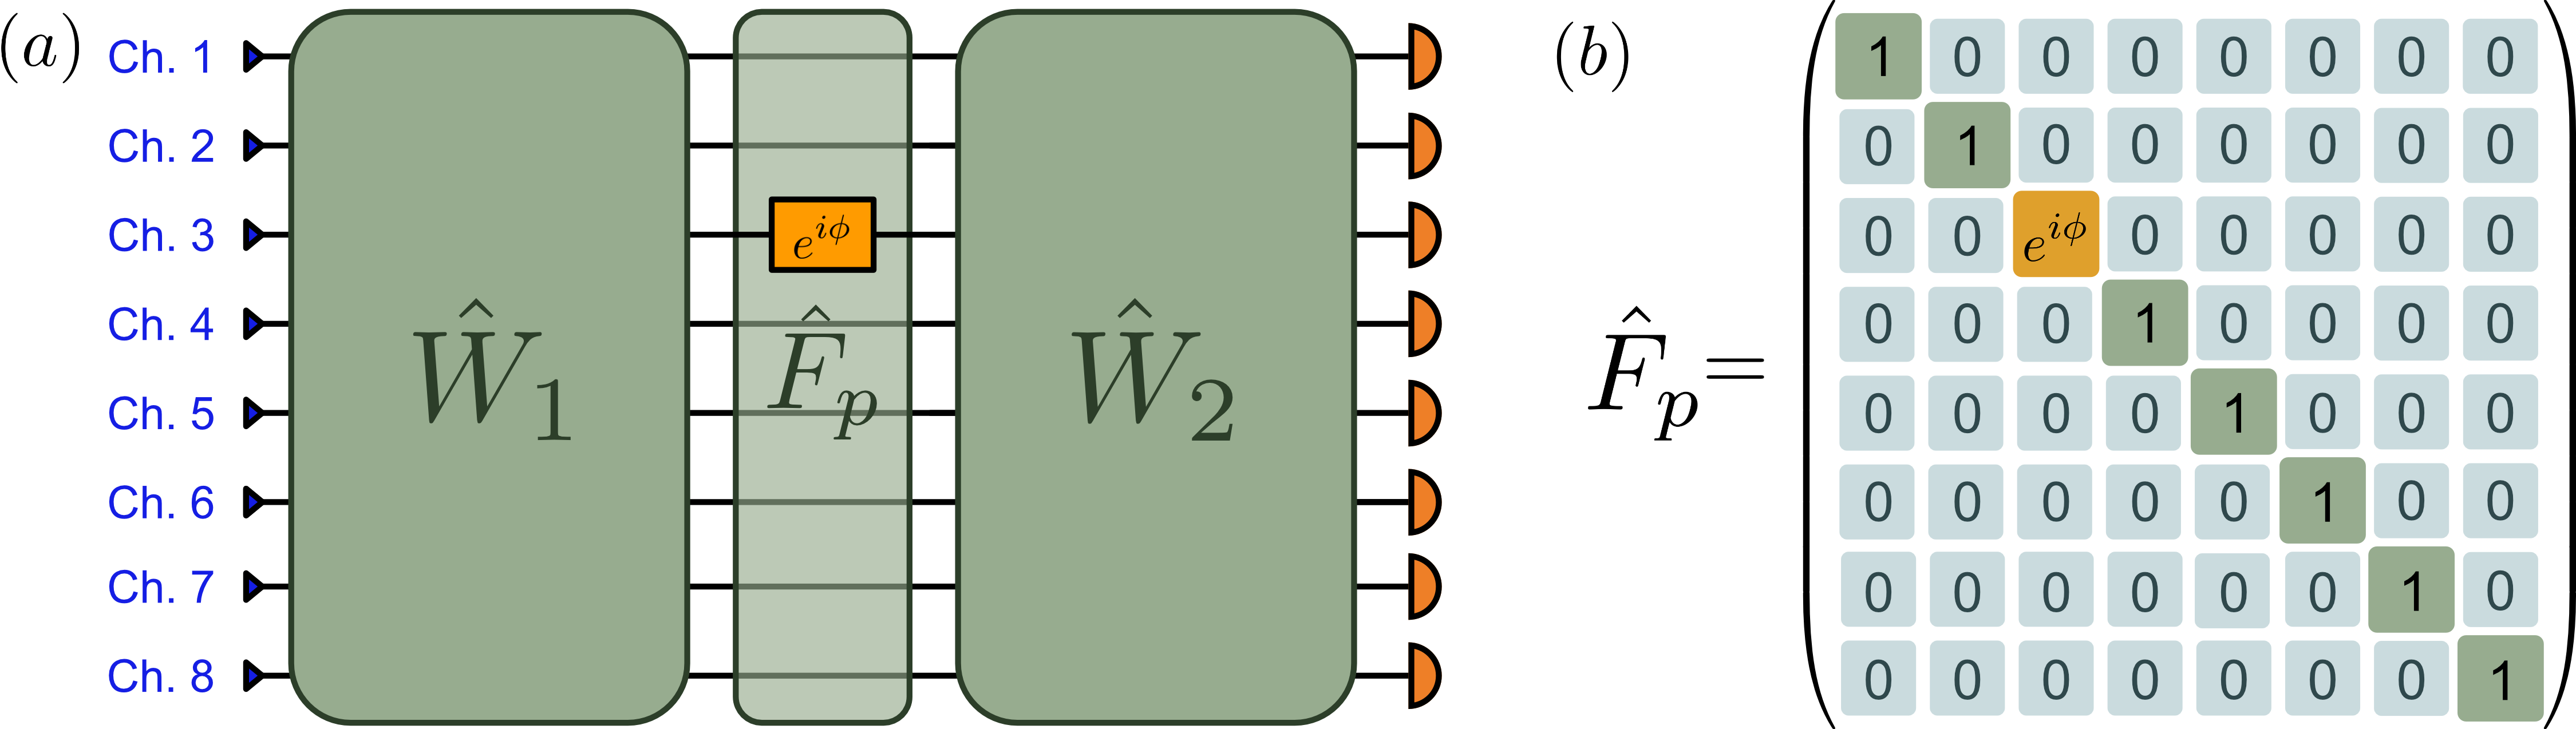
\includegraphics[width=1\linewidth]{images/BlockZerlegungver3.png}
    \caption{(a) Partition of the transfer matrix $\hat{W}$ of an eight-channel \gls{mzi} mesh into a preceding mesh $\hat{W}_1$, an isolated layer $\hat{F}_p$ containing only the phase shifter $p$, and a subsequent mesh
    $\hat{W}_2$. 
    (b) Transfer matrix of the isolated layer $\hat{F}_p$, here for a phase shift acting on channel $q=3$.}
    \label{fig:SplitMesh}
\end{figure}

It remains to evaluate the field derivative 
$\mathrm{d}\mathbf{E}_{\mathrm{out}}/\mathrm{d}p$.
For this we isolate the position in the mesh at which $p$ acts. 
Splitting off this artificial layer $\hat{F}_p$ leaves a preceding mesh $\hat{W}_1$ and a subsequent mesh $\hat{W}_2$, as shown in Figure~\ref{fig:SplitMesh},
\begin{align}
    \hat{W} = \hat{W}_{2}\,\hat{F}_{p}\,\hat{W}_{1},
    \qquad
    \bigl(\hat{F}_{p}\bigr)_{kk} =
    \begin{cases}
        e^{ip}, & k=q,\\
        1,      & k\neq q,
    \end{cases}
    \label{eq:split}
\end{align}
where $q$ denotes the channel on which the phase shifter acts. 
Note that $\hat{F}_p$ is not a physical layer of the mesh. 
Each \gls{mzi} contains two phase shifters, so the cut generally runs through a single \gls{mzi}: 
its first beam splitter belongs to $\hat{W}_1$, while the remaining components belong to $\hat{W}_2$.

Differentiating \eqref{eq:split} affects only the $q$-th diagonal entry,
\begin{align*}
    \frac{\mathrm{d}\hat{F}_{p}}{\mathrm{d}p}
    = i\,e^{ip}\,\mathbf{e}_{q}\mathbf{e}_{q}^{\top},
    \quad \text{with}\
    \mathbf{e}_{q}\in\mathbb{R}^{N},\quad
    \bigl(\mathbf{e}_{q}\bigr)_{k}=\delta_{qk},
    %\label{eq:dFdp}
\end{align*}
Since $\hat{W}_1$ and $\hat{W}_2$ are independent of $p$, they act as constants.
The unit vectors $\mathbf{e}_q$ form an outer product that projects onto the single channel $q$,
\begin{align}
    \frac{\mathrm{d}\mathbf{E}_{\mathrm{out}}}{\mathrm{d}p}
    = \hat{W}_{2}\,\frac{\mathrm{d}\hat{F}_{p}}{\mathrm{d}p}\,
      \hat{W}_{1}\mathbf{E}_{0}
    = i\,e^{i p}\;
      \bigl(\hat{W}_{2}\mathbf{e}_{q}\bigr)
      \underbrace{\bigl(\mathbf{e}_{q}^{\top}\hat{W}_{1}\mathbf{E}_{0}\bigr)}
      _{\textstyle \equiv\, A^{\text{before}}_{p}}.
    \label{eq:dEdp}
\end{align}
Grouping the terms this way isolates a scalar. 
The second bracket is the complex field amplitude $A_p^{\text{before}}$ on channel $q$, immediately in front of the phase shifter. 
It is a quantity that the forward pass produces anyway, and on a physical chip its intensity is accessible through non-invasive on-chip monitors \cite{morichettiNonInvasiveOnChipLight2014}.

Inserting \eqref{eq:dEdp} into \eqref{eq:dL/dp-compact} gives a scalar product with $\boldsymbol{\Gamma}$. 
For a scalar, Hermitian conjugation reduces to complex conjugation, which lets us move $\hat{W}_2$ onto the error field,
\begin{align*}
    \boldsymbol{\Gamma}^{\dagger}\hat{W}_{2}\mathbf{e}_{q}
    = \bigl(\boldsymbol{\Gamma}^{*}\bigr)^{\top}\hat{W}_{2}\mathbf{e}_{q}
    = \mathbf{e}_{q}^{\top}\hat{W}_{2}^{\top}\boldsymbol{\Gamma}^{*}
    = \bigl(\hat{W}_{2}^{\top}\boldsymbol{\Gamma}^{*}\bigr)_{q}.
    %\label{eq:transposestep}
\end{align*}
The transpose $\hat{W}_2^{\top}$ describes propagation from the output ports back to the position of $p$. 
This identification rests on reciprocity of the lossless mesh. 
The conjugated error field $\mathbf{\Gamma}^{*}$ is the source injected at the detectors. 
We define its $q$-th component as the adjoint field amplitude,
\begin{align*}
    A_p^{\mathrm{adj}} \equiv
    \bigl(\hat{W}_{2}^{\top}\mathbf{\Gamma}^{*}\bigr)_{q}.
    %\label{eq:core-Aadj}
\end{align*}
Both $A_p^{\text{before}}$ and $A_p^{\mathrm{adj}}$ are amplitudes taken in front of the phase shifter, each with respect to its own direction of propagation. 
Absorbing the phase factor into the forward amplitude, $A_p \equiv e^{ip}A_p^{\text{before}}$, describes the field directly after the component. 
With $\Re\{i\,z\}=-\Im\{z\}$ we arrive at 
\begin{align}
    \frac{\mathrm{d}\mathcal{L}}{\mathrm{d}p}
    = 2\,\Re\left\{ i\,A_p\,A_p^{\mathrm{adj}} \right\}
    = -2\,\Im\left\{ A_p\,A_p^{\mathrm{adj}} \right\}
    \label{eq:final}
\end{align}
which reproduces the result of \cite{hughesTrainingPhotonicNeural2018}, up to
the factor of two absorbed into their definition of the error field.

Equation \eqref{eq:final} is the result we set out to obtain. 
The gradient with respect to $p$ follows from two field amplitudes at a single location, taken once for the forward field $\mathbf{E}_0$ and once for the backward-propagating error field. 
Both fields traverse the entire mesh in a single pass. 
The cost of a complete gradient evaluation is therefore independent of the number of trainable phases, which is what makes the approach attractive for large meshes.
 
On physical hardware one further step would be required. Photo detectors respond to intensity, so the complex amplitudes in \eqref{eq:final} are not directly accessible.
\citeauthor{hughesTrainingPhotonicNeural2018} address this with the time-reversal interference method, which rests on three principles~\cite{hughesTrainingPhotonicNeural2018}. 
Reciprocity of the lossless mesh makes the backward pass a physically realizable propagation. 
Complex conjugation in the frequency domain corresponds to time reversal, which turns the counter-propagating adjoint field into a co-propagating one. 
Interfering it with the forward field then produces an intensity pattern whose cross term is the required overlap, isolated by subtracting the separately measured constant terms:
\begin{align*}
    I_p = \bigl|A_p + (A_p^{\mathrm{adj}})^{*}\bigr|^{2}
        = |A_p|^{2} + |A_p^{\mathrm{adj}}|^{2}
          + 2\,\Re\left\{A_p\,A_p^{\mathrm{adj}}\right\}.
    %\label{eq:interference}
\end{align*}
The present work focuses on the training method rather than on a full simulation of the physical system. 
We therefore read the field amplitudes $A_p$ and $A_p^{\mathrm{adj}}$ directly from the simulated forward and backward passes, which yields the same gradient \eqref{eq:final} without modeling the measurement protocol.

\section{Additional figures}
\label{appendix:graph}

\subsection{Learning rate analysis}
\label{appendix:graph-learningrate}
\begin{figure}[H]
    \centering
    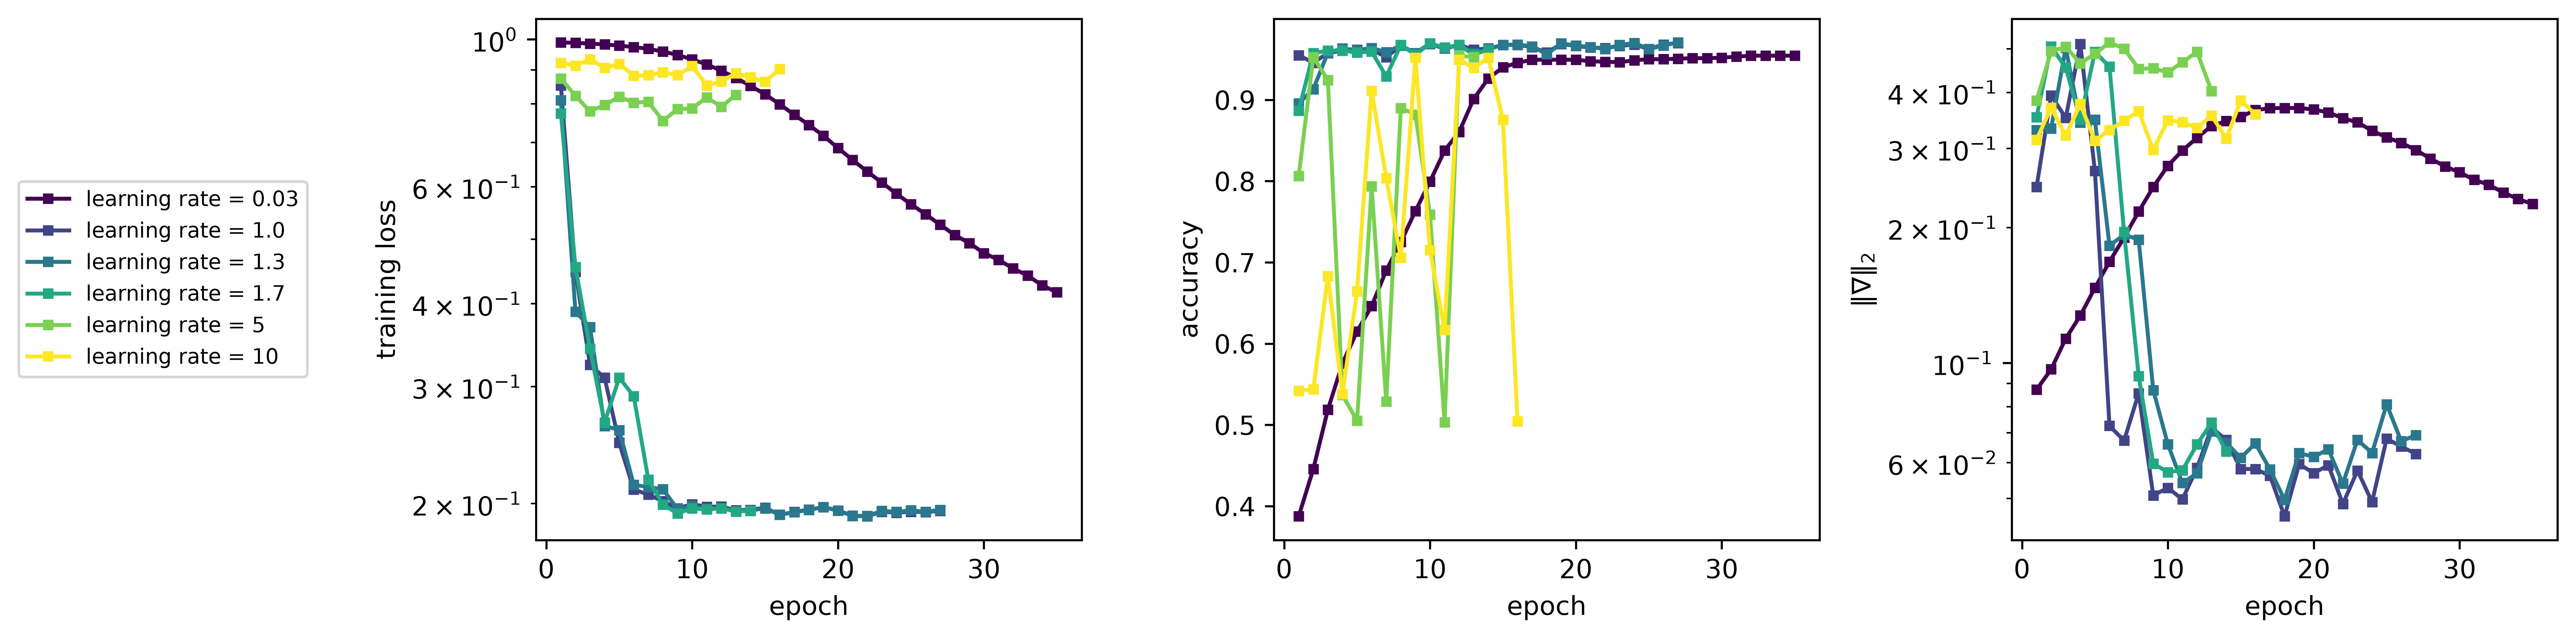
\includegraphics[width=1\linewidth]{evaluation/learning_rate/256_plot_training_epoch.png}
    \caption{Training loss, training accuracy and normalized gradient for different learning rates for a batch size of 256.}
    \label{fig:learning_rate_big_batch_sweep}
\end{figure}

\begin{figure}[H]
    \centering
    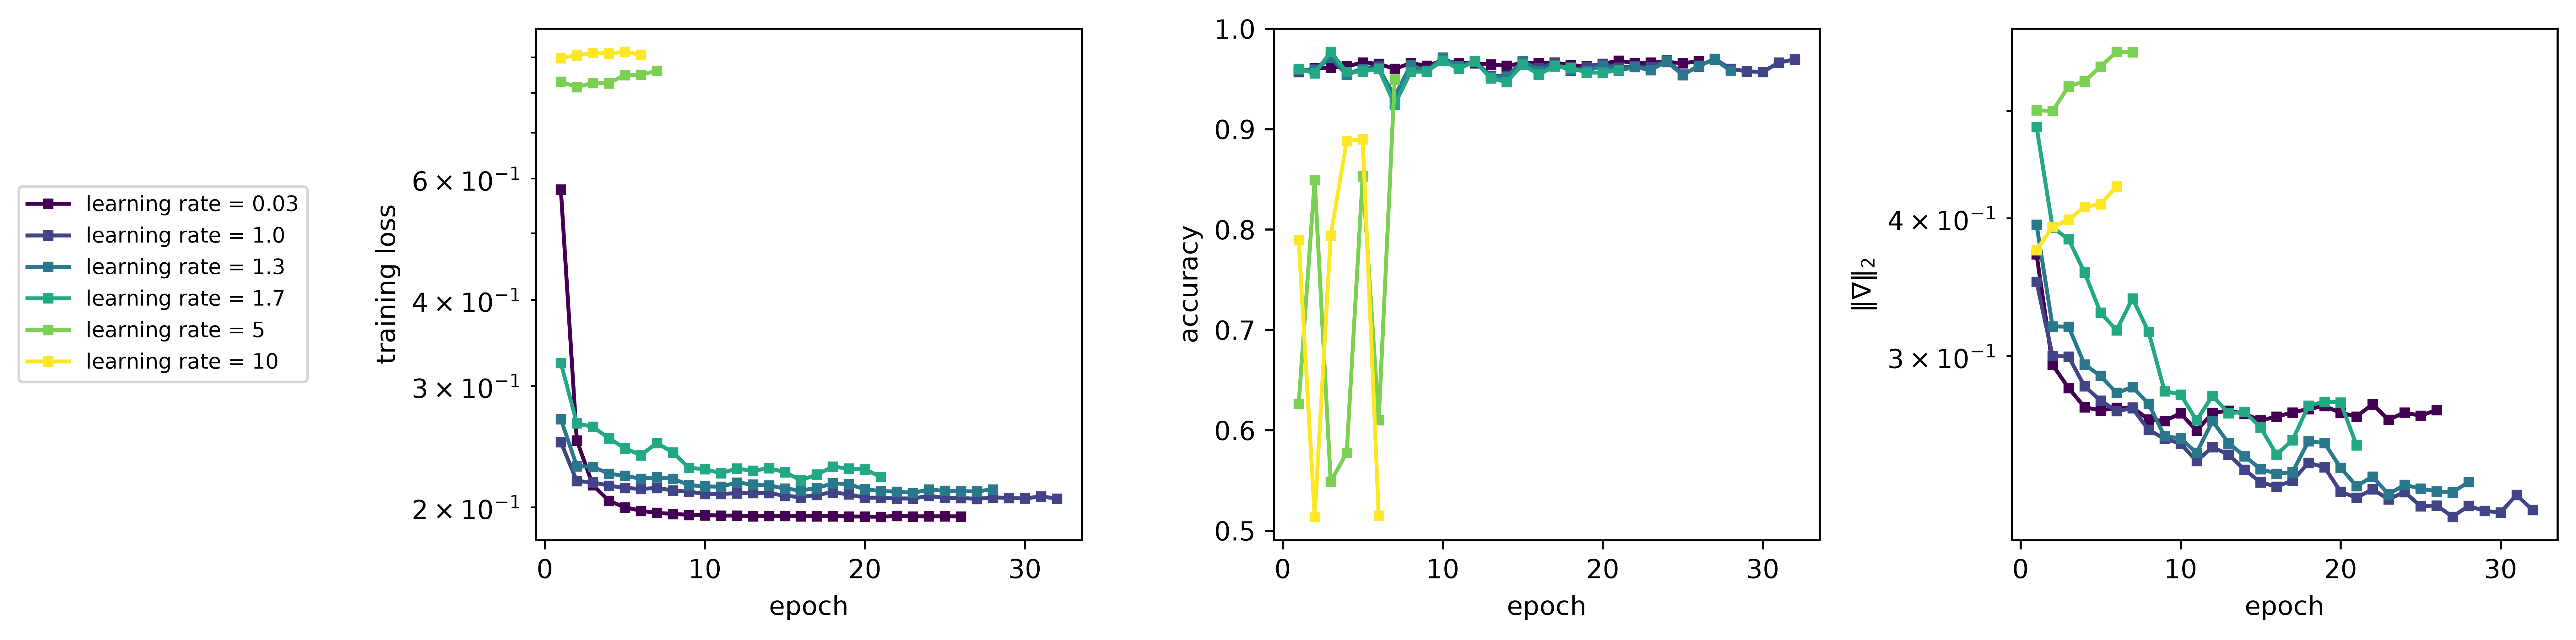
\includegraphics[width=1\linewidth]{evaluation/learning_rate/4_plot_training_epoch.png}
    \caption{Training loss, training accuracy and normalized gradient for different learning rates for a batch size of 4.}
    \label{fig:learning_rate_small_batch_sweep}
\end{figure}

\subsection{Side length analysis (down-sampling)}
\label{appendix:graph-m}
\begin{figure}[H]
    \centering
    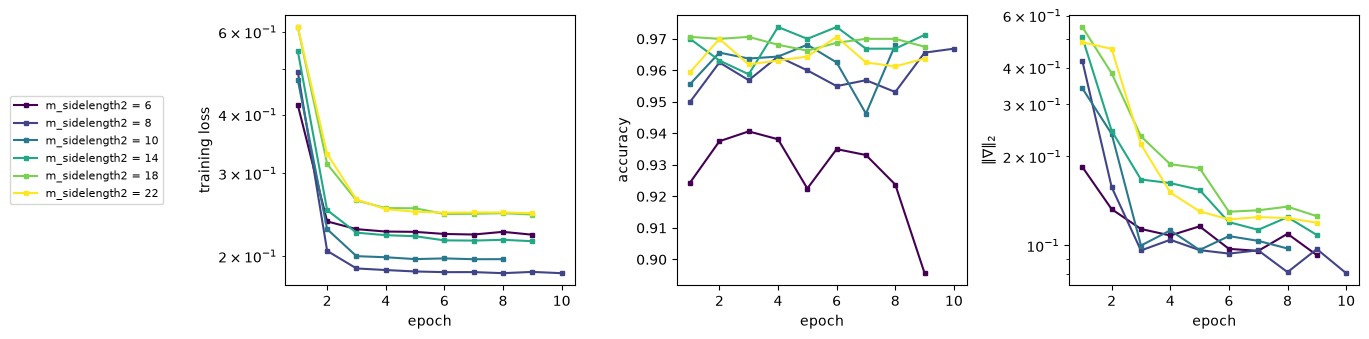
\includegraphics[width=1\linewidth]{evaluation/m_sidelength/plot_training_epoch.png}
    \caption{Training loss, training accuracy and normalized gradient plotted over the epochs for different side lengths of the down-sampled MNIST images.}
    \label{fig:m_sidelength_sweep_epoch}
\end{figure}

\begin{figure}[H]
    \centering
    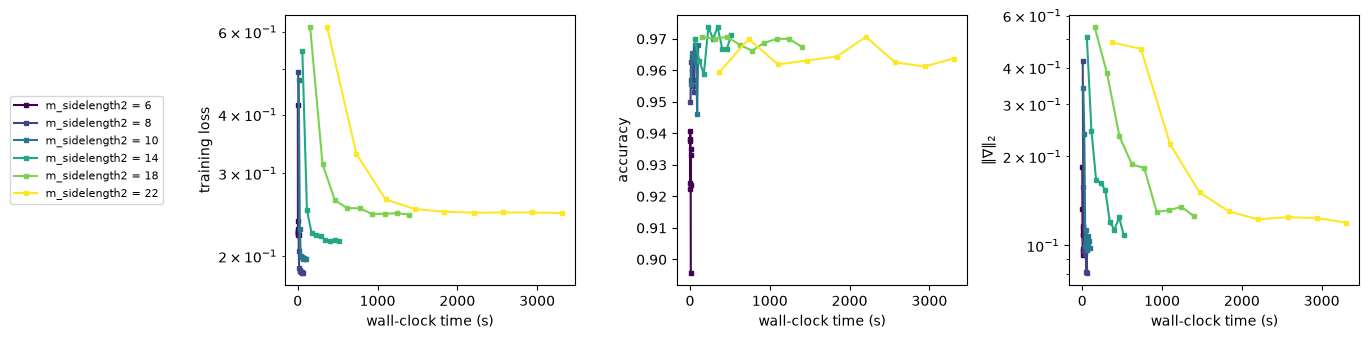
\includegraphics[width=1\linewidth]{evaluation/m_sidelength/plot_training_time.png}
    \caption{Training loss, training accuracy and normalized gradient plotted over the wall-clock time for different side lengths of the down-sampled MNIST images.}
    \label{fig:m_sidelength_sweep_time}
\end{figure}


\subsection{Batch size analysis}
\label{appendix:graph-batchsize}
\begin{figure}[H]
    \centering
    
\includegraphics[width=1\linewidth]{evaluation/batch_size/plot_training_epoch.png}
    \caption{Batch loss, training loss, training accuracy and normalized gradient plotted over the epochs for different batch sizes.}
    \label{fig:batch_size_sweep_epoch}
\end{figure}

\begin{figure}[H]
    \centering
    
\includegraphics[width=1\linewidth]{evaluation/batch_size/plot_training_time.png}
    \caption{Batch loss, training loss, training accuracy and normalized gradient plotted over the wall-clock time for different batch sizes.}
    \label{fig:batch_size_sweep_time}
\end{figure}

\subsection{Hyperparameter theta\_enc (in phase encoding)}
\label{appendix:graph-thetaphase}
\begin{figure}[H]
    \centering
    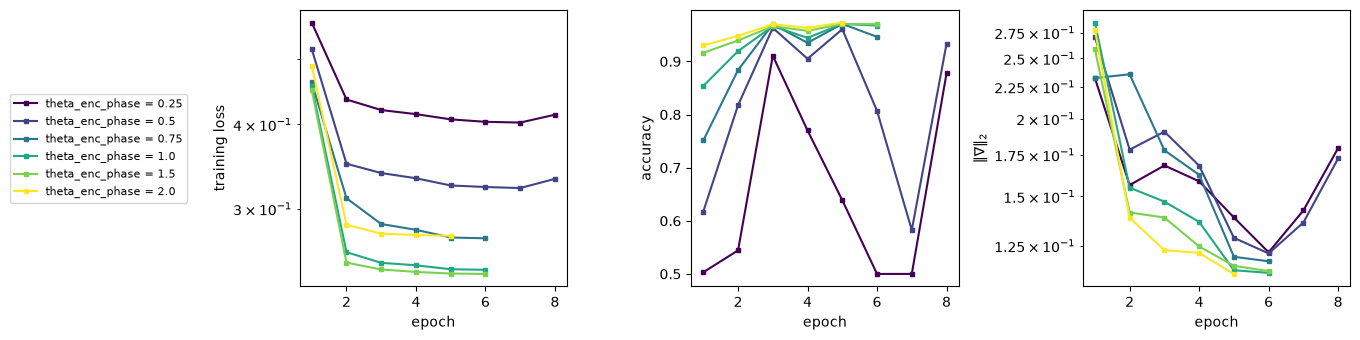
\includegraphics[width=1\linewidth]{evaluation/phase_encoding/output.png}
    \caption{Training loss, training accuracy and normalized gradient plotted over the epochs for different values of \code{theta\_enc} in phase encoding.}
    \label{fig:phase_enc_theta_sweep}
\end{figure}

\subsection{Architecture comparison}
\begin{figure}[H]
    \centering
    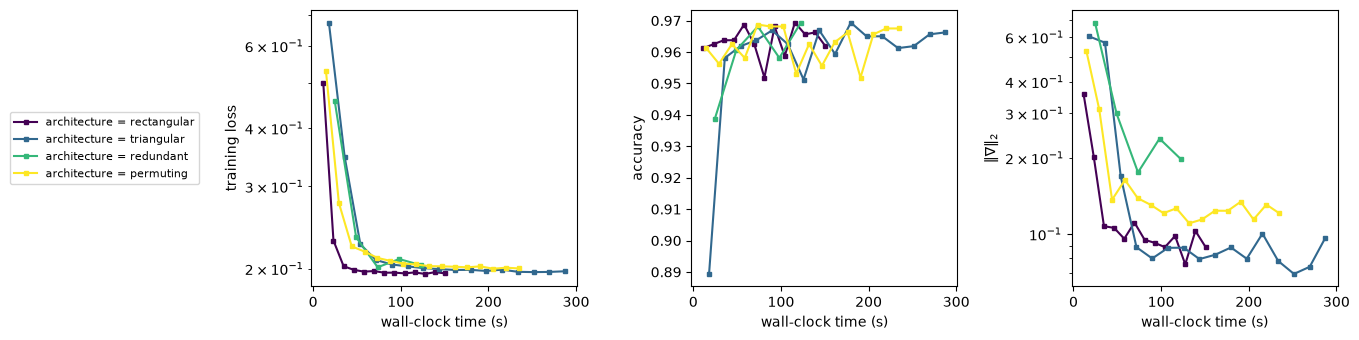
\includegraphics[width=1\linewidth]{evaluation/architecture/output.png}
    \caption{Training loss, training accuracy and normalized gradient for four different architectures of the \gls{mzi} mesh.}
    \label{fig:architecture_sweep}
\end{figure}

\end{appendices}

\end{document}
